\documentclass[11pt]{article}

\usepackage[T1]{fontenc}
\usepackage{lmodern}
\usepackage[margin=1in]{geometry}
\usepackage{microtype}
\usepackage{amsmath,amssymb,mathtools}
\usepackage{booktabs,longtable,array}
\usepackage{graphicx}
\usepackage{pdflscape}
\usepackage{enumitem}
\usepackage{xcolor}
\usepackage{caption}
\usepackage{placeins}
\usepackage{float}
\usepackage[colorlinks=true,
            linkcolor=blue!55!black,
            urlcolor=blue!55!black,
            citecolor=blue!55!black]{hyperref}

\graphicspath{{figures/}}
\setlength{\parindent}{0pt}
\setlength{\parskip}{0.55em}
\setlist{itemsep=0.25em,topsep=0.35em}
\captionsetup{font=small,labelfont=bf}
\renewcommand{\arraystretch}{1.16}

\newcommand{\ii}{\mathrm{i}}
\newcommand{\A}{\mathcal{A}}
\newcommand{\Res}{\operatorname*{Res}}
\newcommand{\QMC}{\mathrm{QMC}}

\title{Sphere \texorpdfstring{$1\to n$}{1 to n} Amplitudes in the
       \texorpdfstring{$c=1$}{c=1} String\\[0.4em]
       \large A numerical worldsheet note}
\author{}
\date{25 August 2026}

\begin{document}
\maketitle

\begin{abstract}
This note records the normalization, soft-energy factorization, contour
prescription, and numerical evidence for the sphere $1\to3$, $1\to4$, and
$1\to5$ tachyon amplitudes in the $c=1$ string.  All three calculations are performed
directly from the worldsheet on the imaginary-energy ray $\omega=\ii t$.
For $1\to3$, all thirty production points lie in the subtraction-free and
residue-free chamber $0<t<1/2$: the original sixteen-point scan is augmented
by fourteen interlaced points computed with the same numerical design.  For
$1\to4$, the original eighteen-point table is augmented by twelve new
worldsheet evaluations to give thirty stored points.  Twenty-nine points
through $t=0.48$ enter the primary quadratic fit; the inherited $t=0.49$
near-second-wall point remains a diagnostic.  The crossed DOZZ residue is
included above the first Liouville-momentum wall, and the merged scan and
worldsheet-only fits are frozen before the matrix-model comparison.  For
$1\to5$, the calculation is restricted to the residue-free chamber
$0<t<1/3$.  The current result uses thirty target-blind Cannon points and
raises the block treatment from order six to order eight through paired
common-Sobol differences.  The order-eight values and cubic fit are fixed
before the matrix-model formula is imported.  The earlier sixteen-point
local scan is retained as an independent historical cross-check.  The
audited data support
\begin{equation*}
  \mu^2\A^{\mathrm{tree}}_{1\to3}(\omega)
  =3\ii\omega^4(1+3\ii\omega),
\end{equation*}
\begin{equation*}
  \mu^3\A^{\mathrm{tree}}_{1\to4}(\omega)
  =8\ii\omega^5(1+2\ii\omega)(1+4\ii\omega)
\end{equation*}
and
\begin{equation*}
  \mu^4\A^{\mathrm{tree}}_{1\to5}(\omega)
  =5\ii\omega^6(1+5\ii\omega)(2+5\ii\omega)(3+5\ii\omega).
\end{equation*}
We also state the expected $1\to n$ formula and outline a scalable
momentum-integration strategy.  The arbitrary-multiplicity formula remains a
comparison target rather than a general worldsheet proof.
\end{abstract}

\tableofcontents

\section{Scope and status}

There are three numerical claims and one general extrapolation in this note.

\begin{enumerate}
  \item The sphere $1\to3$ amplitude has been recomputed at thirty points
  with $0.16\leq t\leq0.46$.  Fourteen new interlaced values were merged with
  the original frozen sixteen-point table without discarding any known datum.
  The raw convergent worldsheet correlator and its affine fits were frozen
  before the separate matrix-model comparison.  Independent deep-scramble
  runs and changes of block and momentum quadrature parameters audit the
  quoted result.

  \item The sphere $1\to4$ amplitude now has a thirty-point stored table:
  twelve new values are merged with all eighteen known values.  The primary
  target-free quadratic fit uses the twenty-nine points through $t=0.48$;
  the known $t=0.49$ near-wall diagnostic is retained but excluded.  The
  calculation has been checked against changes of momentum quadrature,
  Virasoro-block order, quasi-Monte Carlo depth, and OPE channel.  Above the
  first contour wall, the required DOZZ residue is included.  The merged
  worldsheet table and fits were hash-frozen before the separate matrix-model
  comparison.

  \item The current sphere $1\to5$ result consists of thirty points
  $t=0.1805+0.005k$, $k=0,\ldots,29$, all below the first residue wall.  A
  full-statistics order-six mean is corrected by the paired order-eight
  minus order-six shift evaluated on identical Sobol points.  A target-free
  cubic fit is written and hashed before a separate matrix-model comparison.
  The mixed comb--star atlas and three-dimensional Liouville-momentum
  quadrature are unchanged.  The earlier sixteen-point local scan remains
  in the note as an independent cross-check.  No formal order-eight-to-higher
  convergence certificate is claimed, and the proposed order-ten upgrade is
  postponed.

  \item The compact formula for arbitrary $1\to n$ scattering remains the
  analytic expectation suggested by target-space considerations.  The
  $n=3$, $n=4$, and $n=5$ cases now have direct numerical worldsheet evidence, but a
  proof for unrestricted $n$ has not been supplied.
\end{enumerate}

This distinction matters: numerical samples can identify a low-degree
rational or polynomial answer only after one supplies an independent bound
on its analytic form.

\section{Common worldsheet normalization}

Let $I_{n+1}$ denote the labelled sphere matter integral for one incoming and
$n$ outgoing tachyons.  In the BRY normalization,
\begin{equation}
  \A^{\mathrm{tree}}_{1\to n}
  =\ii\bigl(g_s^{\mathrm{BRY}}\bigr)^{n+1}C_{S^2}I_{n+1},
  \qquad
  C_{S^2}=\frac{2\pi}{\bigl(g_s^{\mathrm{BRY}}\bigr)^2}.
  \label{eq:bry-normalization}
\end{equation}
Using
\begin{equation}
  2\pi g_s^{\mathrm{BRY}}=\mu^{-1},
\end{equation}
one obtains
\begin{equation}
  \boxed{
  \mu^{n-1}\A^{\mathrm{tree}}_{1\to n}
  =\ii(2\pi)^{2-n}I_{n+1}.}
  \label{eq:labelled-normalization}
\end{equation}
There is no factor of $1/n!$ in \eqref{eq:labelled-normalization}: the
outgoing insertions are labelled before the equal-energy specialization is
imposed.

After extracting the universal external soft factors, define a stripped
quantity $Q_n$ by
\begin{equation}
  \boxed{
  \mu^{n-1}\A^{\mathrm{tree}}_{1\to n}
  =\ii\omega_{\mathrm{in}}
   \prod_{a=1}^{n}\omega_a\,
   Q_n(\omega_{\mathrm{in}};\omega_1,\ldots,\omega_n).}
  \label{eq:define-Qn}
\end{equation}
No matrix-model expression is needed to define either $I_{n+1}$ or $Q_n$.
In each process-specific section, the target-space formula is therefore
postponed until after the worldsheet integrand, imaginary-energy integration,
and frozen numerical results have been presented.

\section{Why the external powers of energy can be divided out}
\label{sec:soft-factors}

For the delta-normalized $c=25$ Liouville structure constant,
\begin{equation}
  C(P_1,P_2,P_3)\ \propto\
  \prod_{j=1}^{3}2P_j\,\Upsilon_1(1+2\ii P_j),
  \qquad \Upsilon_1(1)=1.
  \label{eq:dozz-soft}
\end{equation}
An external soft limit therefore contributes
\begin{equation}
  C\sim 2P_{\mathrm{ext}}=\omega_{\mathrm{ext}}.
\end{equation}
In a trivalent sphere decomposition, every external leg occurs in exactly
one three-point coefficient.  Provided that the remaining moduli and
Liouville-momentum integrals contain no compensating infrared pole, the full
amplitude contains the product
\begin{equation}
  \omega_{\mathrm{in}}\prod_{a=1}^{n}\omega_a.
  \label{eq:external-soft-product}
\end{equation}

For equal-energy $1\to4$ scattering, this factor is
\begin{equation}
  (4\omega)\omega^4=4\omega^5.
\end{equation}
Thus the factor $\omega^4$ comes from the four outgoing external legs; the
fifth soft factor, $4\omega$, comes from the incoming leg.  This is a
\emph{multiplicative factorization}.  It is not the subtraction of an
$\omega^4$ term from the amplitude.  The caveat about a possible
compensating infrared pole is precisely why the Liouville momentum integral
must be controlled before using this division.

\section{The sphere \texorpdfstring{$1\to3$}{1 to 3} amplitude}
\label{sec:one-to-three}

\subsection{Worldsheet moduli integrand and normalization}

For equal outgoing energies,
\begin{equation}
  (\omega_{\mathrm{in}};\omega_1,\omega_2,\omega_3)
  =(3\omega;\omega,\omega,\omega),
\end{equation}
the labelled normalization and stripped function are
\begin{equation}
  \mu^2\A^{\mathrm{tree}}_{1\to3}=\frac{\ii I_4}{2\pi},
  \qquad
  Q_3(\omega)=\frac{I_4}{6\pi\omega^4},
  \qquad
  \mu^2\A^{\mathrm{tree}}_{1\to3}=3\ii\omega^4Q_3(\omega).
  \label{eq:define-Q3}
\end{equation}
The worldsheet integral has one complex modulus and one internal Liouville
momentum.  In an $s$-channel frame it is
\begin{equation}
 \begin{split}
 I_4(\omega)={}&\int_{\mathbb C}d^2z
 \int_0^\infty\frac{dP}{\pi}\,
 C\left(\frac{3\omega}{2},\frac{\omega}{2},P\right)
 C\left(\frac{\omega}{2},\frac{\omega}{2},P\right)\\
 &\hspace{2.5em}\times
 \mathcal I_{X^0}^{(4)}(z,\bar z;3\omega,-\omega,-\omega,-\omega)
 \left|\mathcal F_{25}^{(4)}(P;z)\right|^2 .
 \end{split}
 \label{eq:I4-worldsheet-integrand}
\end{equation}
Here $\mathcal I_{X^0}^{(4)}$ includes the timelike free-boson and
gauge-fixed ghost powers, and $\mathcal F_{25}^{(4)}$ is the $c=25$
Virasoro block in the chosen crossing frame.  The momentum coefficient is
\begin{equation}
 C\left(\frac{3\omega}{2},\frac{\omega}{2},P\right)
 C\left(\frac{\omega}{2},\frac{\omega}{2},P\right),
 \qquad P\in[0,\infty),
 \label{eq:Q3-DOZZ-product}
\end{equation}
with measure $dP/\pi$ fixed by the delta-normalized Liouville states.

\subsubsection{Convergent chamber and exact three-chart proposal}

On $\omega=\ii t$, the first pair of DOZZ poles capable of pinching the
quotient contour is
\begin{equation}
  P_\pm=\pm(2\omega-\ii),
\end{equation}
so the first residue wall is $t=1/2$.  Near any of the three boundary
divisors $z=0,1,\infty$, the leading local radial behavior at fixed $P$ is
\begin{equation}
 d^2z\,|z|^{-2+2t^2+2P^2}
 \sim dr\,r^{-1+2t^2+2P^2}d\theta.
 \label{eq:Q3-boundary-power}
\end{equation}
It is integrable for every production value $t>0$.  Therefore the
$1\to3$ imaginary-ray computation uses the raw correlator: no BRY finite
part, collar subtraction, or residue term is present.

The moduli proposal is an equal mixture of power-law discs around the three
cusps.  With radial power $a=2t^2$, its exact density with respect to $d^2z$
is
\begin{equation}
 p_a(z)=\frac{a}{6\pi}\left[
 \mathbf 1_{|z|<1}|z|^{a-2}
 +\mathbf 1_{|1-z|<1}|1-z|^{a-2}
 +\mathbf 1_{|z|>1}|z|^{-a-2}\right].
 \label{eq:Q3-three-chart-proposal}
\end{equation}
Every sample is divided by the full mixture density, rather than only by the
density of the chart that generated it.  This makes the estimator unbiased
on overlaps.  Crossing covariance under $z\mapsto1-z$ and $z\mapsto1/z$ was
checked pointwise at relative precision between $10^{-16}$ and $10^{-15}$.

The production settings were block order 10, two Gauss--Legendre momentum
panels with 24 nodes per panel, $P_{\max}=8$, eight independent scrambled
Sobol replicates, and $2^{13}$ moduli points per replicate.  The imaginary
part of the raw result is at most of relative machine precision throughout
the scan.

\subsection{Imaginary-energy worldsheet integration}

The original sixteen-point worldsheet table was augmented by fourteen
interlaced points
\begin{equation}
 t=0.17,0.19,\ldots,0.43.
\end{equation}
These fill the first fourteen gaps of the original
$t=0.16,0.18,\ldots,0.46$ grid; the unused midpoint $t=0.45$ is the one
nearest the residue wall.  Every known datum is retained.  The extension uses
the same block order, momentum quadrature, cutoff, Sobol depth, and replicate
count as the original scan.  Its seed stream begins after the sixteen known
points, so its randomized scrambles are disjoint.  The extension and merged
table, respectively, have SHA-256 hashes
\begin{center}
\small\ttfamily
eaa6a8f131922efed3cdd6029fa83ec98fc9c50ed43c5b7a68a139428e5fa87f,
\\
ab785a09a9d57c68d1e84f12c7c738e83cfaae5fa9b4d7021afd2e4ac1e5a3b9.
\end{center}

The worldsheet-only affine fitter was then run and frozen, still without any
matrix-model coefficient.  The fit artifact has SHA-256 hash
\begin{center}
\small\ttfamily
c0acd1b43a9858c1187967b0ced75f6a383761b68a60fd9ff260e22be5fb274a.
\end{center}
The primary unweighted fit to all thirty production points is
\begin{equation}
  Q_3(\ii t)=0.999774(87)-2.999429(274)t,
  \qquad \mathrm{RMS}=1.2655\times10^{-4}.
  \label{eq:Q3-blind-fit}
\end{equation}
The fourteen new points alone give the sharper cohort diagnostic
\begin{equation}
  Q_3(\ii t)=0.999958(76)-2.999979(243)t,
  \qquad \mathrm{RMS}=6.7992\times10^{-5}.
  \label{eq:Q3-new-cohort-fit}
\end{equation}
Replacing the five previously audited known points by independent
$12\times2^{14}$ deep-scramble evaluations gives the thirty-point
sensitivity fit
\begin{equation}
  Q_3(\ii t)=0.999900(50)-2.999776(158)t,
  \qquad \mathrm{RMS}=7.2742\times10^{-5}.
  \label{eq:Q3-deep-fit}
\end{equation}
The uncertainties in parentheses come from the residual scatter of the
corresponding worldsheet cohort, not from the matrix-model curve.

\subsection{Post-freeze comparison with the matrix model}

Only after the merged scan, worldsheet fits, and convergence audits were
frozen was the comparison function evaluated.  It is
\begin{equation}
  Q_3^{\mathrm{expected}}(\omega)=1+3\ii\omega,
  \qquad
  \boxed{\mu^2\A^{\mathrm{tree}}_{1\to3}(\ii t)
  =3\ii t^4(1-3t).}
  \label{eq:A13-result}
\end{equation}
The fourteen new points alone give $\chi^2_{\QMC}=15.85/14$ against this
curve, with maximum absolute pull $2.38$ and RMS difference
$7.66\times10^{-5}$.  For the complete table, using the five independent
deep values and assigning each a conservative error equal to the largest of
the production error, deep-scramble error, and independent spread gives
$\chi^2=35.56/30$, again with maximum pull $2.38$.  The raw production
replicate errors alone give $\chi^2=66.18/30$ and maximum pull $5.16$.  This
excess is inherited from the known $t=0.32$ point, whose unusually small
production replicate error was already shown to undercover the independent
scramble fluctuation.  The deep result there is
$Q_3(0.32\ii)=0.03999302(520)$, while changes of block order, momentum order,
and cutoff move the answer by less than $2\times10^{-9}$.

{\scriptsize
\begin{longtable}{@{}r c r r r r@{}}
\caption{Frozen thirty-point sphere $1\to3$ worldsheet data.  K and N denote
the sixteen known and fourteen new points.  The expected column was added
only after the merged table and worldsheet-only fits were frozen.}
\label{tab:one-to-three-data}\\
\toprule
$t$ & set & $Q_3^{\mathrm{WS}}$ & $\sigma_{Q,\QMC}$
& $Q_3^{\mathrm{expected}}$ & $\operatorname{Im}(\mu^2\A^{\mathrm{WS}})$ \\
\midrule
\endfirsthead
\multicolumn{6}{c}{\tablename\ \thetable\ continued}\\
\toprule
$t$ & set & $Q_3^{\mathrm{WS}}$ & $\sigma_{Q,\QMC}$
& $Q_3^{\mathrm{expected}}$ & $\operatorname{Im}(\mu^2\A^{\mathrm{WS}})$ \\
\midrule
\endhead
\midrule
\multicolumn{6}{r}{continued on next page}\\
\endfoot
\bottomrule
\endlastfoot
0.16 & K & $+0.519331219$ & $2.93\times10^{-4}$ & $+0.520000$ & $+1.021046722\times10^{-3}$ \\
0.17 & N & $+0.489879571$ & $2.22\times10^{-4}$ & $+0.490000$ & $+1.227456951\times10^{-3}$ \\
0.18 & K & $+0.459910868$ & $1.88\times10^{-4}$ & $+0.460000$ & $+1.448388097\times10^{-3}$ \\
0.19 & N & $+0.430099451$ & $1.00\times10^{-4}$ & $+0.430000$ & $+1.681529718\times10^{-3}$ \\
0.20 & K & $+0.400084688$ & $1.82\times10^{-4}$ & $+0.400000$ & $+1.920406501\times10^{-3}$ \\
0.21 & N & $+0.369961806$ & $1.93\times10^{-4}$ & $+0.370000$ & $+2.158516259\times10^{-3}$ \\
0.22 & K & $+0.339818677$ & $1.25\times10^{-4}$ & $+0.340000$ & $+2.388136920\times10^{-3}$ \\
0.23 & N & $+0.309863956$ & $1.02\times10^{-4}$ & $+0.310000$ & $+2.601379176\times10^{-3}$ \\
0.24 & K & $+0.279826079$ & $1.01\times10^{-4}$ & $+0.280000$ & $+2.785187318\times10^{-3}$ \\
0.25 & N & $+0.249955713$ & $6.79\times10^{-5}$ & $+0.250000$ & $+2.929168511\times10^{-3}$ \\
0.26 & K & $+0.220072276$ & $7.51\times10^{-5}$ & $+0.220000$ & $+3.017032448\times10^{-3}$ \\
0.27 & N & $+0.189899868$ & $8.45\times10^{-5}$ & $+0.190000$ & $+3.027617265\times10^{-3}$ \\
0.28 & K & $+0.159940247$ & $3.87\times10^{-5}$ & $+0.160000$ & $+2.949246968\times10^{-3}$ \\
0.29 & N & $+0.130023447$ & $4.02\times10^{-5}$ & $+0.130000$ & $+2.758893410\times10^{-3}$ \\
0.30 & K & $+0.099992502$ & $3.26\times10^{-5}$ & $+0.100000$ & $+2.429817789\times10^{-3}$ \\
0.31 & N & $+0.069981942$ & $1.26\times10^{-5}$ & $+0.070000$ & $+1.938893786\times10^{-3}$ \\
0.32 & K & $+0.039966050$ & $6.58\times10^{-6}$ & $+0.040000$ & $+1.257223232\times10^{-3}$ \\
0.33 & N & $+0.009998147$ & $3.69\times10^{-6}$ & $+0.010000$ & $+3.557103766\times10^{-4}$ \\
0.34 & K & $-0.020000341$ & $2.54\times10^{-6}$ & $-0.020000$ & $-8.018152530\times10^{-4}$ \\
0.35 & N & $-0.049994040$ & $1.54\times10^{-5}$ & $-0.050000$ & $-2.250669169\times10^{-3}$ \\
0.36 & K & $-0.079970675$ & $2.53\times10^{-5}$ & $-0.080000$ & $-4.029600775\times10^{-3}$ \\
0.37 & N & $-0.109978317$ & $3.15\times10^{-5}$ & $-0.110000$ & $-6.183512183\times10^{-3}$ \\
0.38 & K & $-0.140003033$ & $3.76\times10^{-5}$ & $-0.140000$ & $-8.757760933\times10^{-3}$ \\
0.39 & N & $-0.170048919$ & $3.58\times10^{-5}$ & $-0.170000$ & $-1.180194427\times10^{-2}$ \\
0.40 & K & $-0.200066847$ & $4.13\times10^{-5}$ & $-0.200000$ & $-1.536513382\times10^{-2}$ \\
0.41 & N & $-0.229987890$ & $3.60\times10^{-5}$ & $-0.230000$ & $-1.949672432\times10^{-2}$ \\
0.42 & K & $-0.260080552$ & $5.03\times10^{-5}$ & $-0.260000$ & $-2.427874840\times10^{-2}$ \\
0.43 & N & $-0.290147842$ & $6.20\times10^{-5}$ & $-0.290000$ & $-2.975873200\times10^{-2}$ \\
0.44 & K & $-0.319929356$ & $4.75\times10^{-5}$ & $-0.320000$ & $-3.597377819\times10^{-2}$ \\
0.46 & K & $-0.379961069$ & $4.34\times10^{-5}$ & $-0.380000$ & $-5.103776908\times10^{-2}$ \\
\end{longtable}
}

\begin{figure}[p]
  \centering
  
\includegraphics[width=0.94\textwidth]{results/sphere_four_point_1to3/blind30_20260824/amplitude_comparison_30point.png}
  \caption{Sphere $1\to3$ on $\omega=\ii t$.  Orange circles are the sixteen
  known production points, green diamonds the fourteen new interlaced points,
  and blue squares the five independent deep audits with conservative errors.
  The black curve is the matrix-model expression evaluated only after the
  thirty-point scan and worldsheet fits were frozen.  The panels show $Q_3$,
  the imaginary part of the normalized amplitude, and the pointwise
  worldsheet-minus-matrix difference.}
  \label{fig:one-to-three-comparison}
\end{figure}
\FloatBarrier

\section{The sphere \texorpdfstring{$1\to4$}{1 to 4} amplitude}

\subsection{Worldsheet moduli integrand and normalization}

For the equal-energy kinematics
\begin{equation}
  (\omega_{\mathrm{in}};\omega_1,\omega_2,\omega_3,\omega_4)
  =(4\omega;\omega,\omega,\omega,\omega),
\end{equation}
the two-complex-dimensional worldsheet integral in any chosen trivalent
channel has the form
\begin{equation}
 I_5(\omega)=\int_{\mathcal M_{0,5}}d\mu_5
 \int_0^\infty\frac{dP_1}{\pi}\frac{dP_2}{\pi}\,
 \mathcal I_{X^0}^{(5)}
 \prod_{v=1}^{3}C_{\mathrm L}^{(v)}
 \left|\mathcal F_{25}^{(5)}(P_1,P_2;q_1,q_2)\right|^2 .
 \label{eq:I5-worldsheet-integrand}
\end{equation}
Here $d\mu_5$ is the gauge-fixed moduli measure including the chart
Jacobian, the three $C_{\mathrm L}^{(v)}$ are the delta-normalized Liouville
structure constants, and $\mathcal I_{X^0}^{(5)}$ is the timelike factor for
signed energies $(4\omega,-\omega,-\omega,-\omega,-\omega)$.
We define
\begin{equation}
  Q_4(\omega)=\frac{I_5}{16\pi^2\omega^5}.
  \label{eq:define-Q4}
\end{equation}
The normalized amplitude is then
\begin{equation}
  \mu^3\A^{\mathrm{tree}}_{1\to4}
  =\frac{\ii I_5}{4\pi^2}
  =4\ii\omega^5 Q_4(\omega).
  \label{eq:A-Q4}
\end{equation}

\subsection{Imaginary-energy worldsheet integration}

The direct integration is performed on $\omega=\ii t$.  The conversion from
the stripped worldsheet result to the normalized amplitude follows from
\eqref{eq:A-Q4} alone:
\begin{equation}
  \mu^3\A(\ii t)=-4t^5Q_4(\ii t),
  \qquad
  \sigma_A=4t^5\sigma_Q.
  \label{eq:error-conversion}
\end{equation}

\subsubsection{Numerical values}

The frozen eighteen-point table was augmented by twelve direct worldsheet
evaluations at
\begin{equation}
 t=0.19,0.21,0.23,0.27,0.29,0.31,0.33,0.35,0.37,0.39,0.44,0.47.
\end{equation}
Every known point is retained, including the special probes at $t=0.249$ and
$0.251$ and the $t=0.49$ diagnostic.  The new design avoids the exact
structure-constant zero at $t=1/4$, the first contour wall at $t=2/5$, and
the second wall at $t=1/2$.  All new points use momentum order 20,
$P_{\max}=6$, the threshold-adapted rule $P=6u^{5/4}$, four independent
scrambled Sobol replicates, and the $c$-recursion block.  The extension and
merged worldsheet table have SHA-256 hashes
\begin{center}
\small\ttfamily
be9af08cbd871f727ef6068167fb27467f18428013eaa6a9b9d2fee8e03c584c,
\\
63e8df62c1301110f4131b846dc2908a18a62500564f5a0a891dd90d01f360d1.
\end{center}

The full thirty-point data are given in Table~\ref{tab:numerical-data}.
K and N denote the eighteen known and twelve new points.  The expected
column was evaluated only after the merged table and target-free fits were
frozen.  Quoted standard errors are QMC replicate errors; the independent
block-order spreads at three representative new points enter only the later
conservative comparison.

\begin{landscape}
\begin{center}
\scriptsize
\begin{longtable}{@{}r c r r r r l@{}}
\caption{Frozen thirty-point sphere $1\to4$ dataset.  The final row is the
near-second-wall diagnostic and is excluded from the primary fit.}
\label{tab:numerical-data}\\
\toprule
$t$ & set & $Q_4^{\mathrm{WS}}(\ii t)$ & $\sigma_{Q,\QMC}$
& $Q_4^{\mathrm{expected}}$ & $\mu^3\A^{\mathrm{WS}}(\ii t)$
& Prescription \\
\midrule
\endfirsthead
\multicolumn{7}{c}{\tablename\ \thetable\ (continued)}\\
\toprule
$t$ & set & $Q_4^{\mathrm{WS}}(\ii t)$ & $\sigma_{Q,\QMC}$
& $Q_4^{\mathrm{expected}}$ & $\mu^3\A^{\mathrm{WS}}(\ii t)$
& Prescription \\
\midrule
\endhead
\midrule
\multicolumn{7}{r}{Continued on the next page}\\
\endfoot
\bottomrule
\endlastfoot
0.18 & K & $+0.360141905$ & $3.59\times10^{-4}$ & $+0.358400$ & $-2.722050477\times10^{-4}$ & Real \\
0.19 & N & $+0.297868413$ & $7.69\times10^{-4}$ & $+0.297600$ & $-2.950206718\times10^{-4}$ & Real \\
0.20 & K & $+0.240682960$ & $2.83\times10^{-4}$ & $+0.240000$ & $-3.080741891\times10^{-4}$ & Real \\
0.21 & N & $+0.185361345$ & $2.67\times10^{-4}$ & $+0.185600$ & $-3.028137817\times10^{-4}$ & Real \\
0.22 & K & $+0.134607326$ & $1.68\times10^{-4}$ & $+0.134400$ & $-2.774866497\times10^{-4}$ & Real \\
0.23 & N & $+0.086355703$ & $1.24\times10^{-4}$ & $+0.086400$ & $-2.223259708\times10^{-4}$ & Real \\
0.24 & K & $+0.041592765$ & $4.09\times10^{-5}$ & $+0.041600$ & $-1.324750207\times10^{-4}$ & Real \\
0.249 & K & $+0.004014571$ & $3.94\times10^{-6}$ & $+0.004016$ & $-1.537077710\times10^{-5}$ & Real \\
0.251 & K & $-0.003982449$ & $3.91\times10^{-6}$ & $-0.003984$ & $+1.587006931\times10^{-5}$ & Real \\
0.26 & K & $-0.038411505$ & $5.16\times10^{-5}$ & $-0.038400$ & $+1.825526146\times10^{-4}$ & Real \\
0.27 & N & $-0.073604833$ & $1.94\times10^{-4}$ & $-0.073600$ & $+4.224595627\times10^{-4}$ & Real \\
0.28 & K & $-0.105602511$ & $1.49\times10^{-4}$ & $-0.105600$ & $+7.269832315\times10^{-4}$ & Real \\
0.29 & N & $-0.134252025$ & $2.00\times10^{-4}$ & $-0.134400$ & $+1.101465313\times10^{-3}$ & Real \\
0.30 & K & $-0.159973349$ & $2.38\times10^{-4}$ & $-0.160000$ & $+1.554940955\times10^{-3}$ & Real \\
0.31 & N & $-0.182339671$ & $3.06\times10^{-4}$ & $-0.182400$ & $+2.088091993\times10^{-3}$ & Real \\
0.32 & K & $-0.201535953$ & $3.18\times10^{-4}$ & $-0.201600$ & $+2.704969768\times10^{-3}$ & Real \\
0.33 & N & $-0.216868021$ & $5.17\times10^{-4}$ & $-0.217600$ & $+3.394886091\times10^{-3}$ & Real \\
0.34 & K & $-0.230229797$ & $2.51\times10^{-4}$ & $-0.230400$ & $+4.184235372\times10^{-3}$ & Real \\
0.35 & N & $-0.242549497$ & $1.40\times10^{-3}$ & $-0.240000$ & $+5.095661747\times10^{-3}$ & Continued; inactive \\
0.36 & K & $-0.247439049$ & $1.71\times10^{-3}$ & $-0.246400$ & $+5.984677245\times10^{-3}$ & Continued; inactive \\
0.37 & N & $-0.250033136$ & $1.44\times10^{-3}$ & $-0.249600$ & $+6.935314814\times10^{-3}$ & Continued; inactive \\
0.38 & K & $-0.250784365$ & $1.82\times10^{-3}$ & $-0.249600$ & $+7.948376520\times10^{-3}$ & Continued; inactive \\
0.39 & N & $-0.247485294$ & $1.18\times10^{-3}$ & $-0.246400$ & $+8.931664969\times10^{-3}$ & Continued; inactive \\
0.395 & K & $-0.244256937$ & $1.85\times10^{-3}$ & $-0.243600$ & $+9.394904648\times10^{-3}$ & Continued; inactive \\
0.42 & K & $-0.218868687$ & $1.74\times10^{-3}$ & $-0.217600$ & $+1.144168732\times10^{-2}$ & Residue corrected \\
0.44 & N & $-0.182612916$ & $6.71\times10^{-4}$ & $-0.182400$ & $+1.204633301\times10^{-2}$ & Residue corrected \\
0.46 & K & $-0.135603621$ & $1.17\times10^{-3}$ & $-0.134400$ & $+1.117173014\times10^{-2}$ & Residue corrected \\
0.47 & N & $-0.105739056$ & $8.75\times10^{-4}$ & $-0.105600$ & $+9.700289781\times10^{-3}$ & Residue corrected \\
0.48 & K & $-0.073467644$ & $6.60\times10^{-4}$ & $-0.073600$ & $+7.487938910\times10^{-3}$ & Residue corrected \\
0.49 & K & $-0.036352662$ & $4.19\times10^{-4}$ & $-0.038400$ & $+4.107490899\times10^{-3}$ & Residue; diagnostic \\
\end{longtable}
\end{center}
\end{landscape}

\subsubsection{Liouville contour continuation}
\label{sec:contour-continuation}

On $\omega=\ii t$, the incoming--outgoing cherry coefficient has the nearest
pair of poles
\begin{equation}
  P_{\pm}=\pm\left(\frac{5}{2}\omega-\ii\right).
  \label{eq:first-poles}
\end{equation}
They pinch the endpoint of the real quotient contour at
\begin{equation}
  t=\frac{2}{5}.
  \label{eq:first-wall}
\end{equation}
For $2/5<t<1/2$, the continued contribution from an internal edge whose
cherry contains both the incoming operator and one outgoing operator is
\begin{equation}
  \int_0^\infty\frac{dP}{\pi}\,I(P)
  -2\ii\Res_{P=(5/2)\omega-\ii}I(P).
  \label{eq:residue-prescription}
\end{equation}
Channels in which the incoming operator sits at the middle vertex receive no
residue at this first wall.

The points at $t=0.35,0.36,0.37,0.38,0.39,0.395$ were evaluated using the
same continued-contour implementation, but the residue term is inactive
below $t=2/5$.  Every stored point above the wall includes the residue term
in \eqref{eq:residue-prescription}.

A second pole family pinches at $t=1/2$.  The first-wall formula cannot be
continued past that value without adding the next residue stratum.  The
$t=0.49$ point is therefore retained as a diagnostic rather than treated as
a production point.

\subsubsection{Worldsheet numerical audit}

The following checks concern worldsheet convergence only.  Their computation
routines do not evaluate or import a matrix-model amplitude.

\begin{enumerate}
  \item At $t=0.34$, momentum orders 20 and 24 gave $-0.2303047302$ and
  $-0.2303034636$, respectively.

  \item At the same point, varying $P_{\max}=5,6,7$ produced a range of only
  $2.6\times10^{-5}$.

  \item Sobol powers 9, 10, and 11 agreed within their QMC errors.

  \item At $t=0.26$, block levels 8 and 10 gave $-0.03849398(20)$ and
  $-0.03836665(22)$; their spread is retained as a block-truncation
  diagnostic.

  \item An equal-quality overlapping-channel test at $t=0.34$ improved from
  a $0.44\%$ mismatch at block level 6 to a $0.069\%$ mismatch at level 8.

  \newpage
  \item Three independent new-point block-order audits were performed after
  the primary fit was frozen.  At $t=0.31$, the production block-6 value
  $-0.18233967$ and block-8 audit $-0.18240429$ differ by
  $6.46\times10^{-5}$.  At $t=0.35$, the block-8 production value
  $-0.24254950$ and block-6 audit $-0.23855076$ differ by
  $4.00\times10^{-3}$.  At the residue-corrected point $t=0.44$, the
  corresponding values $-0.18261292$ and $-0.18098326$ differ by
  $1.63\times10^{-3}$.  The latter two spreads exceed the replicate errors
  and are carried as conservative local uncertainties in the downstream
  comparison.  The frozen audit has SHA-256 hash
  \begin{center}
  \small\ttfamily
  3b3a966dcf215237baae09d5014f47dff735dc2e28c1bb67c68309e8b6a73ce5.
  \end{center}

  \item Independent descendant, $h$-recursion, $c$-recursion, atlas,
  Jacobian, and contour-wall checks passed.
\end{enumerate}

The stored points continue to bracket the first exact zero without evaluating
the logarithmic DOZZ expression at its pole:
\begin{equation}
  Q_4(\ii\,0.249)=0.00401457(39),
  \qquad
  Q_4(\ii\,0.251)=-0.00398245(39).
\end{equation}
At exactly $t=1/4$, the evaluator encounters the corresponding
structure-constant zero, so that coordinate is intentionally absent from the
numerical design.

\subsubsection{Target-free quadratic fit on the imaginary ray}

For analytic continuation from the imaginary-energy chamber, we impose the
explicit degree-two ansatz
\begin{equation}
  Q_4(\ii t)=a+bt+ct^2.
  \label{eq:Q4-fit-ansatz}
\end{equation}
A mechanical extraction first writes a points-only table containing no
matrix-model coefficient.  Its SHA-256 hash is
\begin{center}
\small\ttfamily
611d5f1f75d7fdd0240aaa134803b656f6a157c3928a91cca0e6f4cc85c00a12.
\end{center}
The target-free fitting program uses all twenty-nine points through $t=0.48$,
including the five residue-corrected values at
$t=0.42,0.44,0.46,0.47,0.48$.  The $t=0.49$ near-second-wall diagnostic is
retained in the table but excluded from the primary fit.  Because the stored
pointwise errors do not supply the full correlated block/discretization
covariance, the primary fit is unweighted ordinary least squares.  Its frozen
artifact has SHA-256 hash
\begin{center}
\small\ttfamily
5e165ec33cdbd721af8ce5550212315eb41a07323bad42b7bd83ae7f51e61907.
\end{center}
The result is
\begin{equation}
  \boxed{
  (a,b,c)=
  (2.004567\mathbin{\pm}0.001687,\,
   -12.026247\mathbin{\pm}0.010763,\,
   16.032869\mathbin{\pm}0.016273),}
  \label{eq:Q4-imaginary-fit}
\end{equation}
where the parenthesized errors come from the residual scatter.  The RMS
residual is $6.04\times10^{-4}$ and the largest absolute residual is
$1.96\times10^{-3}$.  The twelve new points alone give the independent cohort
fit
\begin{equation}
  (a,b,c)_{\mathrm{new\,12}}
  =(2.002855\mathbin{\pm}0.003581,\,
    -12.017837\mathbin{\pm}0.022820,\,
    16.023398\mathbin{\pm}0.034654),
  \label{eq:Q4-imaginary-fit-new12}
\end{equation}
with RMS residual $7.47\times10^{-4}$.  The roots of the primary frozen fit
are $t=0.25001494$ and $0.50008459$; the latter is quoted only as the root of
the degree-two reconstruction because the first-wall contour formula is not
validated at the second wall.

\subsection{Post-freeze comparison with the matrix model}

Only after the points-only table and the fit in
\eqref{eq:Q4-imaginary-fit} were written did the downstream program evaluate
the matrix-model coefficients.  The comparison target is
\begin{equation}
  Q_4^{\mathrm{expected}}(\omega)
  =2(1+2\ii\omega)(1+4\ii\omega),
  \qquad
  Q_4^{\mathrm{expected}}(\ii t)=2(1-2t)(1-4t).
  \label{eq:Q4-expected}
\end{equation}
Consequently,
\begin{equation}
  \boxed{
  \mu^3\A^{\mathrm{tree}}_{1\to4}(\omega)
  =8\ii\omega^5(1+2\ii\omega)(1+4\ii\omega),}
  \qquad
  \mu^3\A^{\mathrm{tree}}_{1\to4}(\ii t)
  =-8t^5(1-2t)(1-4t).
  \label{eq:A14-result}
\end{equation}
For the twelve new points, the QMC-only pointwise statistic is
$\chi^2=8.01/12$, with maximum absolute pull $1.82$.  Enlarging the errors at
the three audited new points to the largest of the production QMC error,
audit QMC error, and independent block-order spread gives
$\chi^2=5.00/12$ and maximum pull $1.42$.  The complete twenty-nine-point
primary table gives $\chi^2=42.35/29$ using QMC errors and $39.33/29$ with
the same conservative audit prescription.  Its largest pull, $4.86$, is the
inherited known point at $t=0.18$, not a new datum.

The primary fitted coefficients differ from $(2,-12,16)$ by
$0.228\%$, $0.219\%$, and $0.205\%$, respectively.  Its reconstructed roots
$0.25001494$ and $0.50008459$ agree with the matrix-model roots $1/4$ and
$1/2$ at the stated numerical resolution.  Agreement over a finite set of
points does not by itself prove the quadratic degree; that degree is the
explicit analytic ansatz in \eqref{eq:Q4-fit-ansatz}.  This comparison is an
imaginary-energy analytic-continuation result and does not claim that the
separate direct physical-$\ii\epsilon$ finite-part smoke test is complete.

\begin{figure}[p]
  \centering
  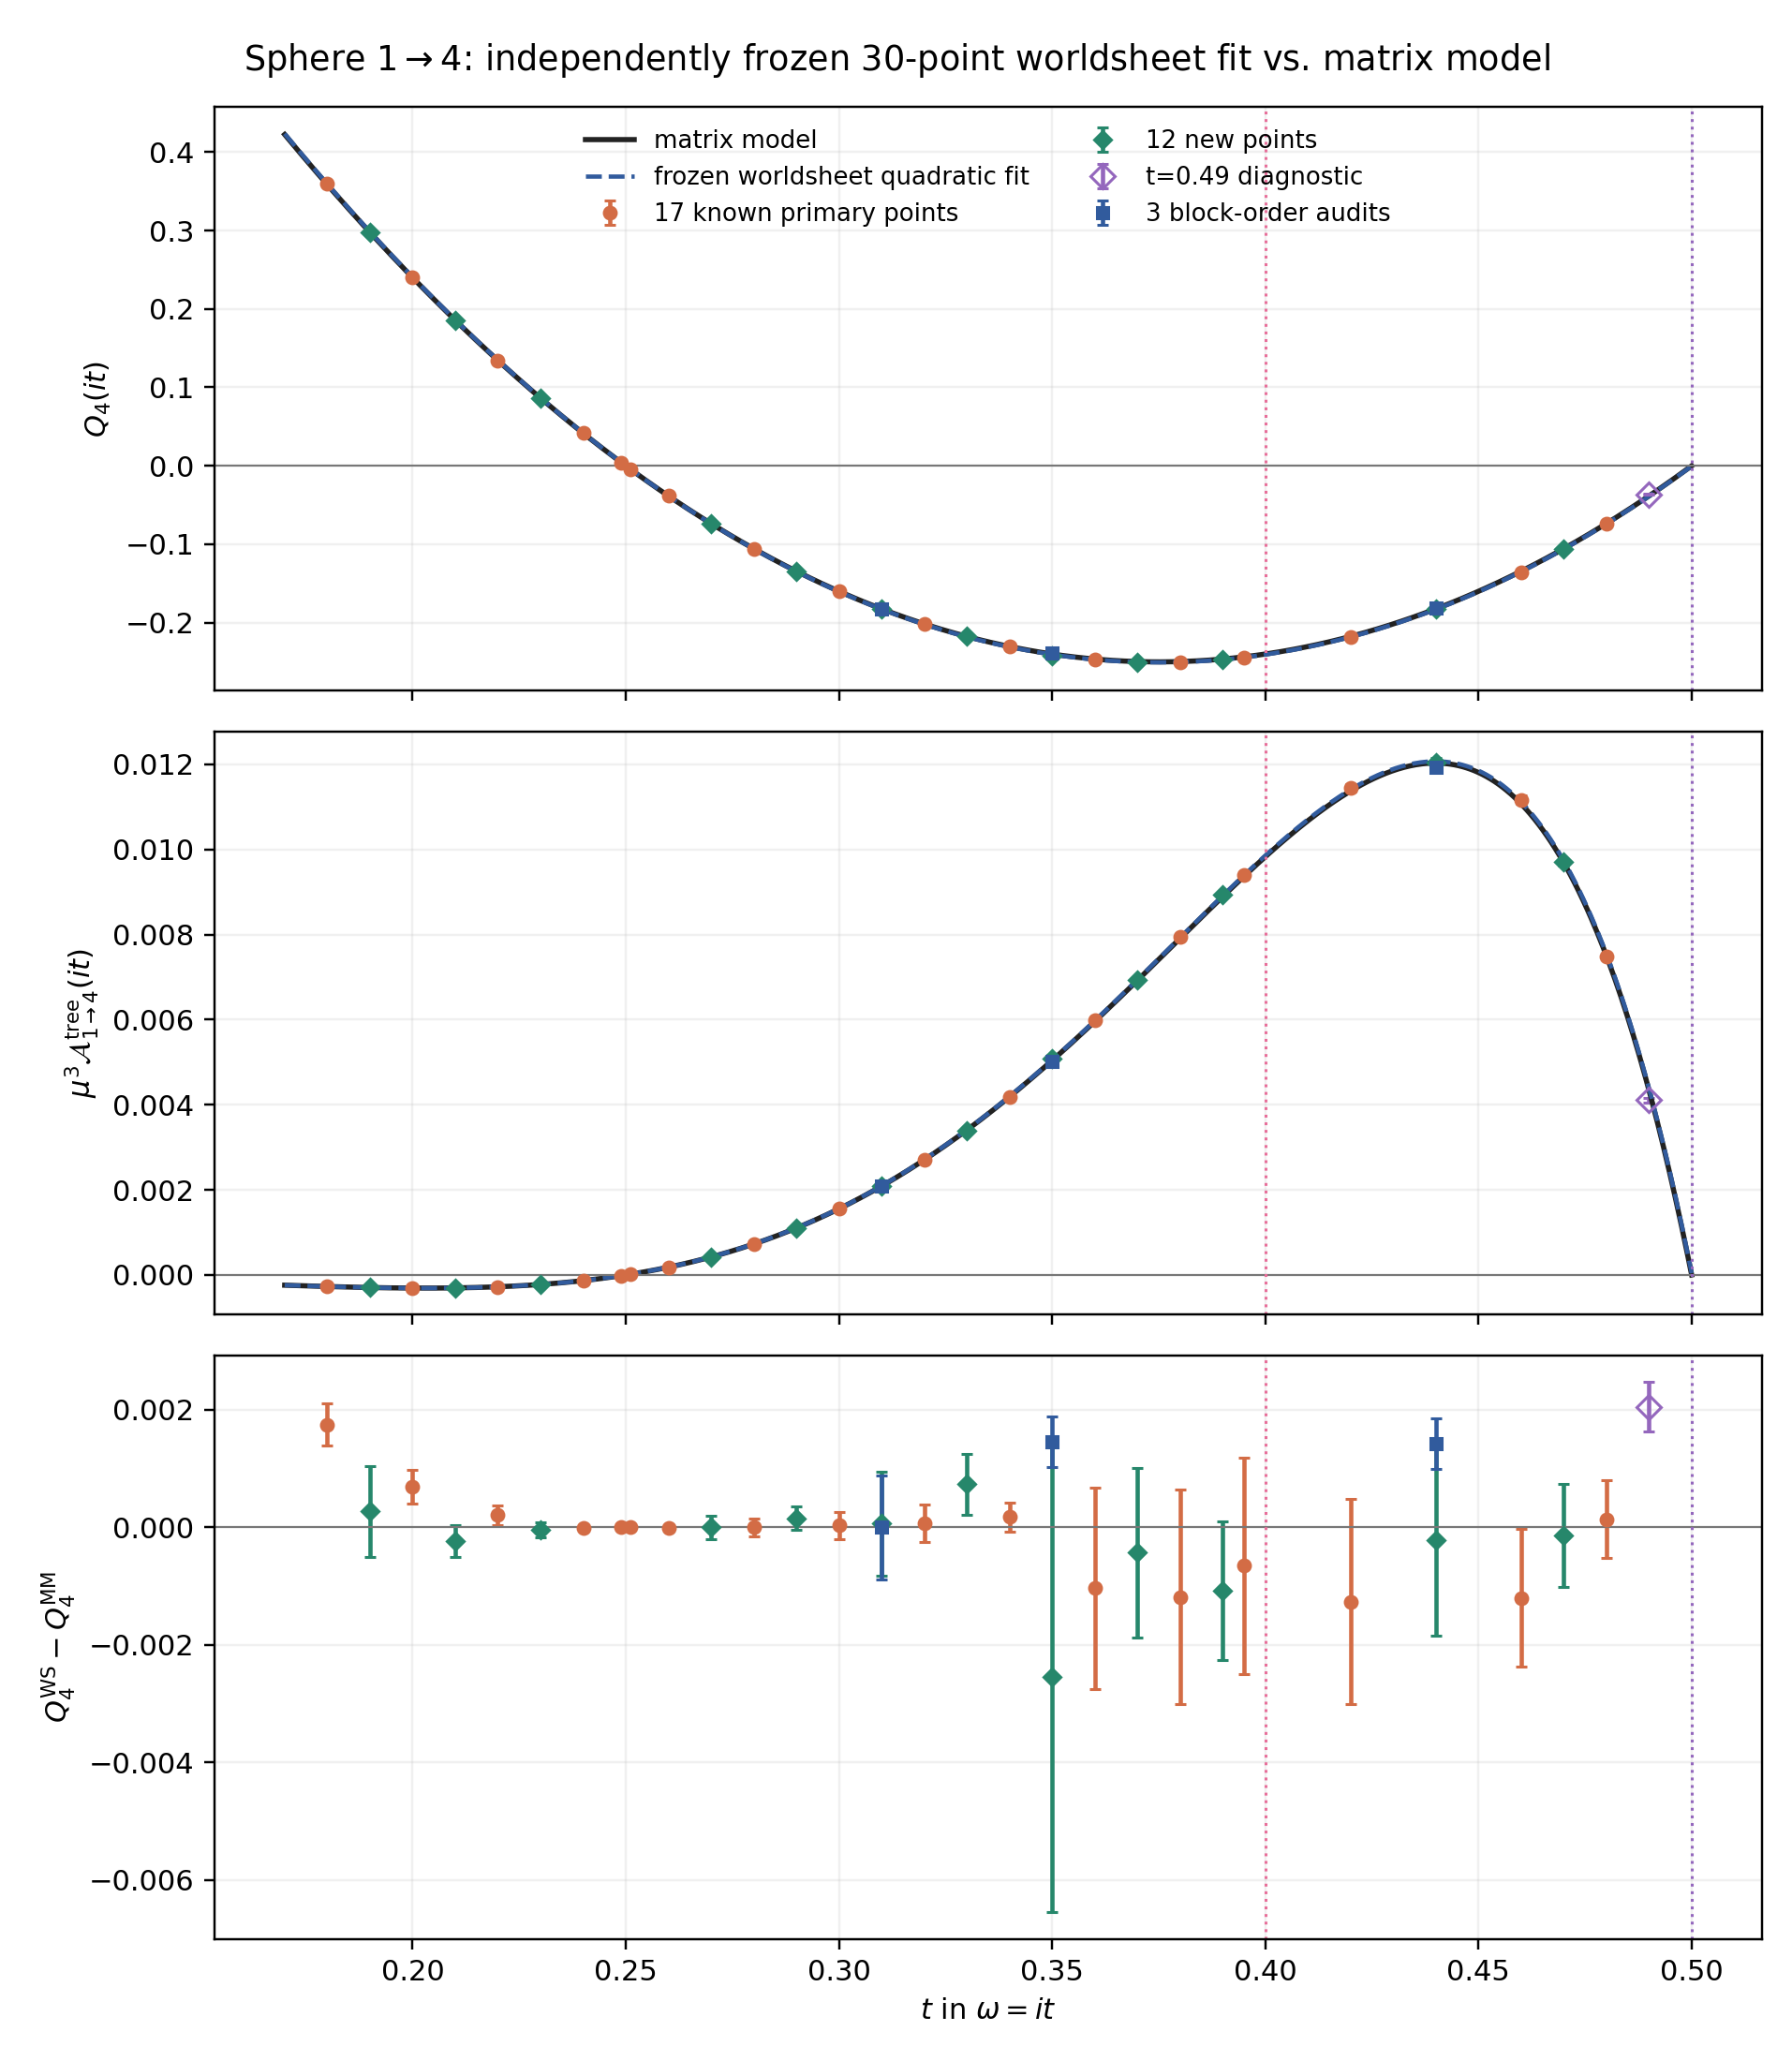
\includegraphics[width=0.84\textwidth]{results/sphere_five_point_1to4/blind30_20260824/amplitude_comparison_30point.png}
  \caption{Sphere $1\to4$ on $\omega=\ii t$.  Orange circles are the
  seventeen known primary points, green diamonds the twelve new points, and
  the open purple diamond the inherited $t=0.49$ near-wall diagnostic.
  Blue squares are the three independent block-order audits.  The black
  curve is the matrix model evaluated after the thirty-point table and
  target-free fits were frozen; the dashed blue curve is the frozen
  twenty-nine-point worldsheet fit.  The panels show $Q_4$, the normalized
  amplitude, and the pointwise worldsheet-minus-matrix difference.  Error
  bars on audited production points use the conservative spread described in
  the text.}
  \label{fig:amplitude-comparison}
\end{figure}
\FloatBarrier
\clearpage

\section{The sphere \texorpdfstring{$1\to5$}{1 to 5} amplitude}
\label{sec:one-to-five}

\subsection{Worldsheet moduli integrand and normalization}

For the equal-energy kinematics
\begin{equation}
  (\omega_{\mathrm{in}};\omega_1,\ldots,\omega_5)
  =(5\omega;\omega,\omega,\omega,\omega,\omega),
\end{equation}
the six-point worldsheet integral in any fixed trivalent channel has the
schematic form
\begin{equation}
  I_6(\omega)=\int_{\mathcal M_{0,6}}d\mu_6
      \int_0^\infty\prod_{j=1}^{3}\frac{dP_j}{\pi}\,
      \mathcal I_{X^0}^{(6)}
      \prod_{v=1}^{4}C_{\mathrm L}^{(v)}
      \left|\mathcal F_{25}^{(6)}
      (P_1,P_2,P_3;q_1,q_2,q_3)\right|^2.
  \label{eq:I6-schematic}
\end{equation}
Here $d\mu_6$ is the gauge-fixed moduli measure including the selected-chart
Jacobian, the four $C_{\mathrm L}^{(v)}$ are delta-normalized Liouville
structure constants, and $\mathcal I_{X^0}^{(6)}$ is the timelike factor for
signed energies $(5\omega,-\omega,-\omega,-\omega,-\omega,-\omega)$.
the labelled normalization \eqref{eq:labelled-normalization} gives
\begin{equation}
  \mu^4\A^{\mathrm{tree}}_{1\to5}
  =\frac{\ii I_6}{8\pi^3}.
  \label{eq:A15-I6}
\end{equation}
The product of external soft factors is $5\omega^6$.  It is therefore useful
to define
\begin{equation}
  Q_5(\omega)=\frac{I_6}{40\pi^3\omega^6},
  \qquad
  \mu^4\A^{\mathrm{tree}}_{1\to5}
  =5\ii\omega^6Q_5(\omega).
  \label{eq:define-Q5}
\end{equation}

\subsubsection{Mixed atlas and channel-dependent six-point block}

The six-point moduli integral is split with an equal mixture of 720 oriented
comb charts and 720 oriented star charts.  After forgetting orientations,
these represent 90 comb trees and 15 star trees.  At every sampled point the
code reconstructs all admissible plumbing coordinates and evaluates the
Virasoro block in the topology with the smallest maximum plumbing radius.
The production scan selected comb and star channels in nearly equal
proportions; the largest selected radius was $0.9027$.

The comb and star six-point blocks were implemented independently.  Their
global limits and their $c$-recursions agree with direct descendant
definitions through the tested orders.  The maximum relative discrepancy in
the comb $c$-recursion tests was $1.2\times10^{-15}$, while the corresponding
star discrepancy was $1.9\times10^{-15}$.  Round trips between moduli and
plumbing coordinates and the complex Jacobians agree at approximately
$10^{-16}$.  A triple-cherry degeneration, which is poorly represented by a
comb, is mapped to star radii as small as $(0.1,0.03,0.01)$.

\subsubsection{Three-dimensional Liouville-momentum integration}

The three internal momenta are mapped as
\begin{equation}
  P_j=P_{\max}u_j^{5/4},
  \qquad 0<u_j<1,
  \qquad P_{\max}=5.
  \label{eq:six-point-momentum-map}
\end{equation}
In the earlier sixteen-point local scan, Gauss--Legendre rules of adjacent
orders $(8,9,10)$ are used on the three
edges.  The unequal orders avoid accidental simultaneous Kac-pole collisions
in the $c$-recursion.  The DOZZ/Yin factors are evaluated logarithmically,
and the complete $P_1P_2P_3$ contraction tensor is cached for reuse in the
moduli integral.  The production block order is four.  Six independently
scrambled Sobol replicates, with 128 moduli points per replicate and radial
CDF $r^{0.2}$, determine the QMC error.  The thirty-point update below keeps
the same momentum map and radial proposal, while raising the base momentum
order to ten, the production block order to six, and the paired block audit
to order eight.

\subsection{Imaginary-energy worldsheet integration}

On the convergent ray $\omega=\ii t$, the normalization above gives
\begin{equation}
  Q_5(\ii t)=-\frac{I_6}{40\pi^3t^6},
  \qquad
  \mu^4\A^{\mathrm{tree}}_{1\to5}(\ii t)
  =-5\ii t^6Q_5(\ii t).
  \label{eq:A15-imaginary-ray}
\end{equation}
The nearest moving pole pair is
\begin{equation}
  P_{\pm}=\pm(3\omega-\ii).
  \label{eq:A15-first-poles}
\end{equation}
It reaches the real momentum contour at
\begin{equation}
  t=\frac13.
  \label{eq:A15-first-wall}
\end{equation}
All production points satisfy $0<t<1/3$.  No pole has crossed any real
$P_j$ contour in this chamber, so no residue term is present.  This is an
analytic statement about the contour, distinct from numerical control of the
ordinary quadrature remainder.  The implementation rejects input outside
this chamber rather than silently omitting residues.

\subsubsection{Earlier sixteen-point blind freeze and numerical audit}

\begin{samepage}
The original eight-point worldsheet scan was completed before any
matrix-model formula was loaded.  Its frozen SHA-256 hash is
\begin{center}
\small\ttfamily
216925ad78f35331a39aadc26d28a83a61bef415509ddfd6df491c127dd0e62a.
\end{center}
\end{samepage}
Eight further local points at
\begin{equation}
 t=0.155,0.180,0.195,0.205,0.210,0.240,0.280,0.320
\end{equation}
were then computed by the same worldsheet-only driver.  The original and
extension tables were merged without changing any value and frozen before a
new sixteen-point comparison.  The merged SHA-256 hash is
\begin{center}
\small\ttfamily
fa8b60ce2bb1c34cec61ba7629f0051d15762d522d0527b5404fc1c4f36be0a6.
\end{center}
At the representative point $t=0.18$, the following shifts in $Q_5$ were
found:
\begin{align}
  (8,9,10)\ \hbox{versus}\ (7,8,9)
    &: 3.43\times10^{-4},\\
  \hbox{block order }4\ \hbox{versus}\ 6
    &: 7.00\times10^{-4},\\
  P_{\max}=5\ \hbox{versus}\ 4
    &: 6.46\times10^{-4}.
\end{align}
Their quadrature sum defines the conservative absolute discretization error
\begin{equation}
  \delta_{\mathrm{disc}}Q_5=1.012\times10^{-3}.
  \label{eq:Q5-discretization}
\end{equation}
An alternate radial sampler shifted $Q_5$ by $0.00729$, within its combined
QMC uncertainty of approximately $0.010$.  It therefore revealed no resolved
importance-sampling bias.  No regulated-block or direct-block fallback was
used at any production point.

\subsubsection{Earlier sixteen-point target-free cubic fit}

Before loading any comparison formula, a mechanical extraction wrote a
points-only table from the frozen sixteen-point scan.  Its SHA-256 hash is
\begin{center}
\small\ttfamily
eeb8243db391dbae895b52823b25bf93ac8168b962e31e79ab062302cb054d6b.
\end{center}
The fitting program contains no matrix-model coefficient.  It assumes only
the explicit analytic ansatz
\begin{equation}
  Q_5(\ii t)=a+bt+ct^2+dt^3.
  \label{eq:Q5-worldsheet-fit-ansatz}
\end{equation}
The primary generalized least-squares covariance treats the scrambled-Sobol
QMC errors as independent and the single discretization estimate in
\eqref{eq:Q5-discretization} as one fully correlated additive nuisance across
all $t$.  The frozen target-free result is
\begin{equation}
\begin{split}
 (a,b,c,d)={}&(6.33158,-58.91205,164.86491,-142.96917),\\
 \sigma_{a,b,c,d}={}&(0.37817,4.88690,20.78288,28.96791),
\end{split}
\label{eq:Q5-worldsheet-cubic-fit}
\end{equation}
with $\chi^2=1.13$ for 12 residual degrees of freedom.  The low value is
consistent with the deliberately conservative error model and should not be
read as evidence that every systematic is statistically independent.

As conditioning diagnostics, the two alternative coefficient vectors are
\begin{align}
 (a,b,c,d)_{\mathrm{diag}}
   &=(6.36015,-59.23433,166.04757,-144.38683),\\
 (a,b,c,d)_{\mathrm{unweighted}}
   &=(7.05086,-67.66480,199.65477,-188.22656).
\end{align}
The first combines the discretization estimate diagonally, while the second
is an ordinary unweighted fit.  The coefficient vector is therefore
less sharply determined than the fitted curve: all points lie in the narrow
interval $0.14\leq t\leq0.32$, and the lowest-$t$ points carry the largest
errors.  The correlated GLS prescription above is fixed as the primary
result; these two alternatives are reported only as sensitivity tests.

\subsubsection{Thirty-point paired order-eight update}

The completed Cannon calculation supplies thirty target-blind worldsheet
points
\begin{equation}
  t_k=0.1805+0.005k,
  \qquad k=0,\ldots,29,
  \label{eq:Q5-order8-grid}
\end{equation}
all strictly below $t=1/3$.  At each point, the full production mean uses
block order six, momentum orders $(10,11,12)$, $P_{\max}=5$, fourteen
independently scrambled Sobol replicates, and $2^{15}$ moduli points per
replicate.  A disjoint six-replicate, $2^{11}$-point stream evaluates block
orders six and eight on identical Sobol points.  The current order-eight
estimator is therefore
\begin{equation}
  \widehat Q_5^{(8)}(t)
  =\overline Q_{5,\mathrm{full}}^{(6)}(t)
   +\overline{\left(Q_5^{(8)}-Q_5^{(6)}\right)}_{\mathrm{paired}}(t),
  \label{eq:Q5-paired-order8-estimator}
\end{equation}
with propagated statistical variance
\begin{equation}
  \left(\sigma_{8,\mathrm{stat}}\right)^2
  =\left(\sigma_{6,\mathrm{full}}\right)^2
   +\left(\sigma_{8-6,\mathrm{paired}}\right)^2.
  \label{eq:Q5-paired-order8-error}
\end{equation}
This construction spends the large sample on the cheaper order-six
integrand and resolves the block correction with a common-random-number
difference.  The independent seed streams justify the variance sum in
\eqref{eq:Q5-paired-order8-error}.  No matrix-model coefficient appears in
either the completed source table or this postprocessor, and all recorded
fallback counts vanish.

The assembled target-blind source has SHA-256 hash
\begin{center}
\small\ttfamily
e460d5de342a61641da662d3f08bef81e2e1759e7220ae8dc365676850f152d7.
\end{center}
The target-free order-eight output has SHA-256 hash
\begin{center}
\small\ttfamily
a021e1165b1c7cfbf6cb852b9ba685454145bcc6e8883cb8e11bc87e327707e5.
\end{center}
Fitting only the ansatz in \eqref{eq:Q5-worldsheet-fit-ansatz}, with the
propagated statistical errors in \eqref{eq:Q5-paired-order8-error}, gives
\begin{equation}
\begin{split}
 (a,b,c,d)={}&(6.21496,-56.88322,154.63270,-127.95294),\\
 \sigma_{a,b,c,d}={}&(0.10398,1.30064,5.35582,7.24154),
\end{split}
\label{eq:Q5-order8-cubic-fit}
\end{equation}
with $\chi^2=2.12$ for 26 residual degrees of freedom, maximum absolute fit
residual $2.08\times10^{-3}$, and RMS residual $9.68\times10^{-4}$.  As a
conditioning check, weighting by the available numerical-envelope proxy
instead gives
\begin{equation}
 (a,b,c,d)_{\mathrm{env}}
 =(6.19841,-56.67403,153.76488,-126.77468),
\end{equation}
while the unweighted fit gives
\begin{equation}
 (a,b,c,d)_{\mathrm{unweighted}}
 =(6.11992,-55.70169,149.86542,-121.69079).
\end{equation}

The original $5\times10^{-4}$ campaign gate was defined as the maximum of
the production QMC error and two-sigma order-six stability shifts.  It did
not pass at all thirty points because the block-order-six to block-order-eight
change was resolved.  Here that resolved change is incorporated into
\eqref{eq:Q5-paired-order8-estimator}.  The stored order-six stability
envelope is retained below as a conservative display and comparison proxy;
it is \emph{not} a formal order-eight-to-higher convergence certificate.
The order-ten upgrade is postponed, and no order-ten datum enters this fit.

\subsection{Post-fit comparison with the matrix model}

Only after both the points-only table and the target-free cubic fit were
frozen was the comparison program allowed to load
\begin{equation}
  \boxed{
  Q_5^{\mathrm{expected}}(\omega)
  =(1+5\ii\omega)(2+5\ii\omega)(3+5\ii\omega).}
  \label{eq:Q5-expected}
\end{equation}
Equivalently,
\begin{equation}
  Q_5^{\mathrm{expected}}(\ii t)
  =(1-5t)(2-5t)(3-5t).
  \label{eq:Q5-expected-it}
\end{equation}
The comparison is summarized in Table~\ref{tab:one-to-five-data}.  The quoted
error is
\begin{equation}
  \sigma_{Q,\mathrm{combined}}
  =\sqrt{\sigma_{Q,\QMC}^2+(\delta_{\mathrm{disc}}Q_5)^2}.
  \label{eq:Q5-combined-error}
\end{equation}

\begin{table}[htbp]
\centering
\small
\caption{The original eight-point core of the frozen sphere $1\to5$
worldsheet data below the first residue wall.
The matrix-model column was evaluated only after the worldsheet file was
frozen.}
\label{tab:one-to-five-data}
\begin{tabular}{@{}r r r r r@{}}
\toprule
$t$ & $Q_5^{\mathrm{WS}}$ & $\sigma_{Q,\mathrm{combined}}$
& $Q_5^{\mathrm{expected}}$ & $\operatorname{Im}(\mu^4\A^{\mathrm{WS}})$ \\
\midrule
0.140 & $ 0.982781$ & $0.102102$ & $ 0.897000$ & $-3.69994\times10^{-5}$ \\
0.170 & $ 0.385419$ & $0.020166$ & $ 0.370875$ & $-4.65154\times10^{-5}$ \\
0.190 & $ 0.109379$ & $0.003641$ & $ 0.107625$ & $-2.57290\times10^{-5}$ \\
0.199 & $ 0.010171$ & $0.001048$ & $ 0.010075$ & $-3.15817\times10^{-6}$ \\
0.201 & $-0.010007$ & $0.001045$ & $-0.009925$ & $ 3.29943\times10^{-6}$ \\
0.220 & $-0.171046$ & $0.003878$ & $-0.171000$ & $ 9.69657\times10^{-5}$ \\
0.260 & $-0.355720$ & $0.008996$ & $-0.357000$ & $ 5.49437\times10^{-4}$ \\
0.300 & $-0.364899$ & $0.011647$ & $-0.375000$ & $ 1.33006\times10^{-3}$ \\
\bottomrule
\end{tabular}
\end{table}

The worldsheet calculation resolves the expected sign change without using
the target formula:
\begin{equation}
  Q_5(\ii\,0.199)=0.010171(1048),
  \qquad
  Q_5(\ii\,0.201)=-0.010007(1045),
\end{equation}
where the parentheses now include both QMC and discretization errors.  In the
original core, all eight points lie within $0.87$ combined standard
deviations of \eqref{eq:Q5-expected-it}, with $\chi^2=2.24/8$.  In the merged
sixteen-point table the maximum absolute diagonal pull is $1.31$.  Treating
the discretization estimate as the correlated nuisance used in the fit gives
$\chi^2=5.61/16$.  The matrix-model coefficient vector
$(6,-55,150,-125)$ differs from the target-free fit by at most $14.4\%$ in an
individual coefficient; every coefficient difference is below $0.88$ of its
marginal fit standard error, and the full correlated coefficient quadratic
form is $4.47$ for four directions.  These are useful diagnostics rather
than formal likelihood statistics.  They show good consistency while also
preserving the conditioning caveat above.  The complete sixteen-point table,
fit covariance, and comparison grid are stored in the machine-readable
artifacts cited in Appendix~\ref{sec:code-map}.

\begin{figure}[p]
  \centering
  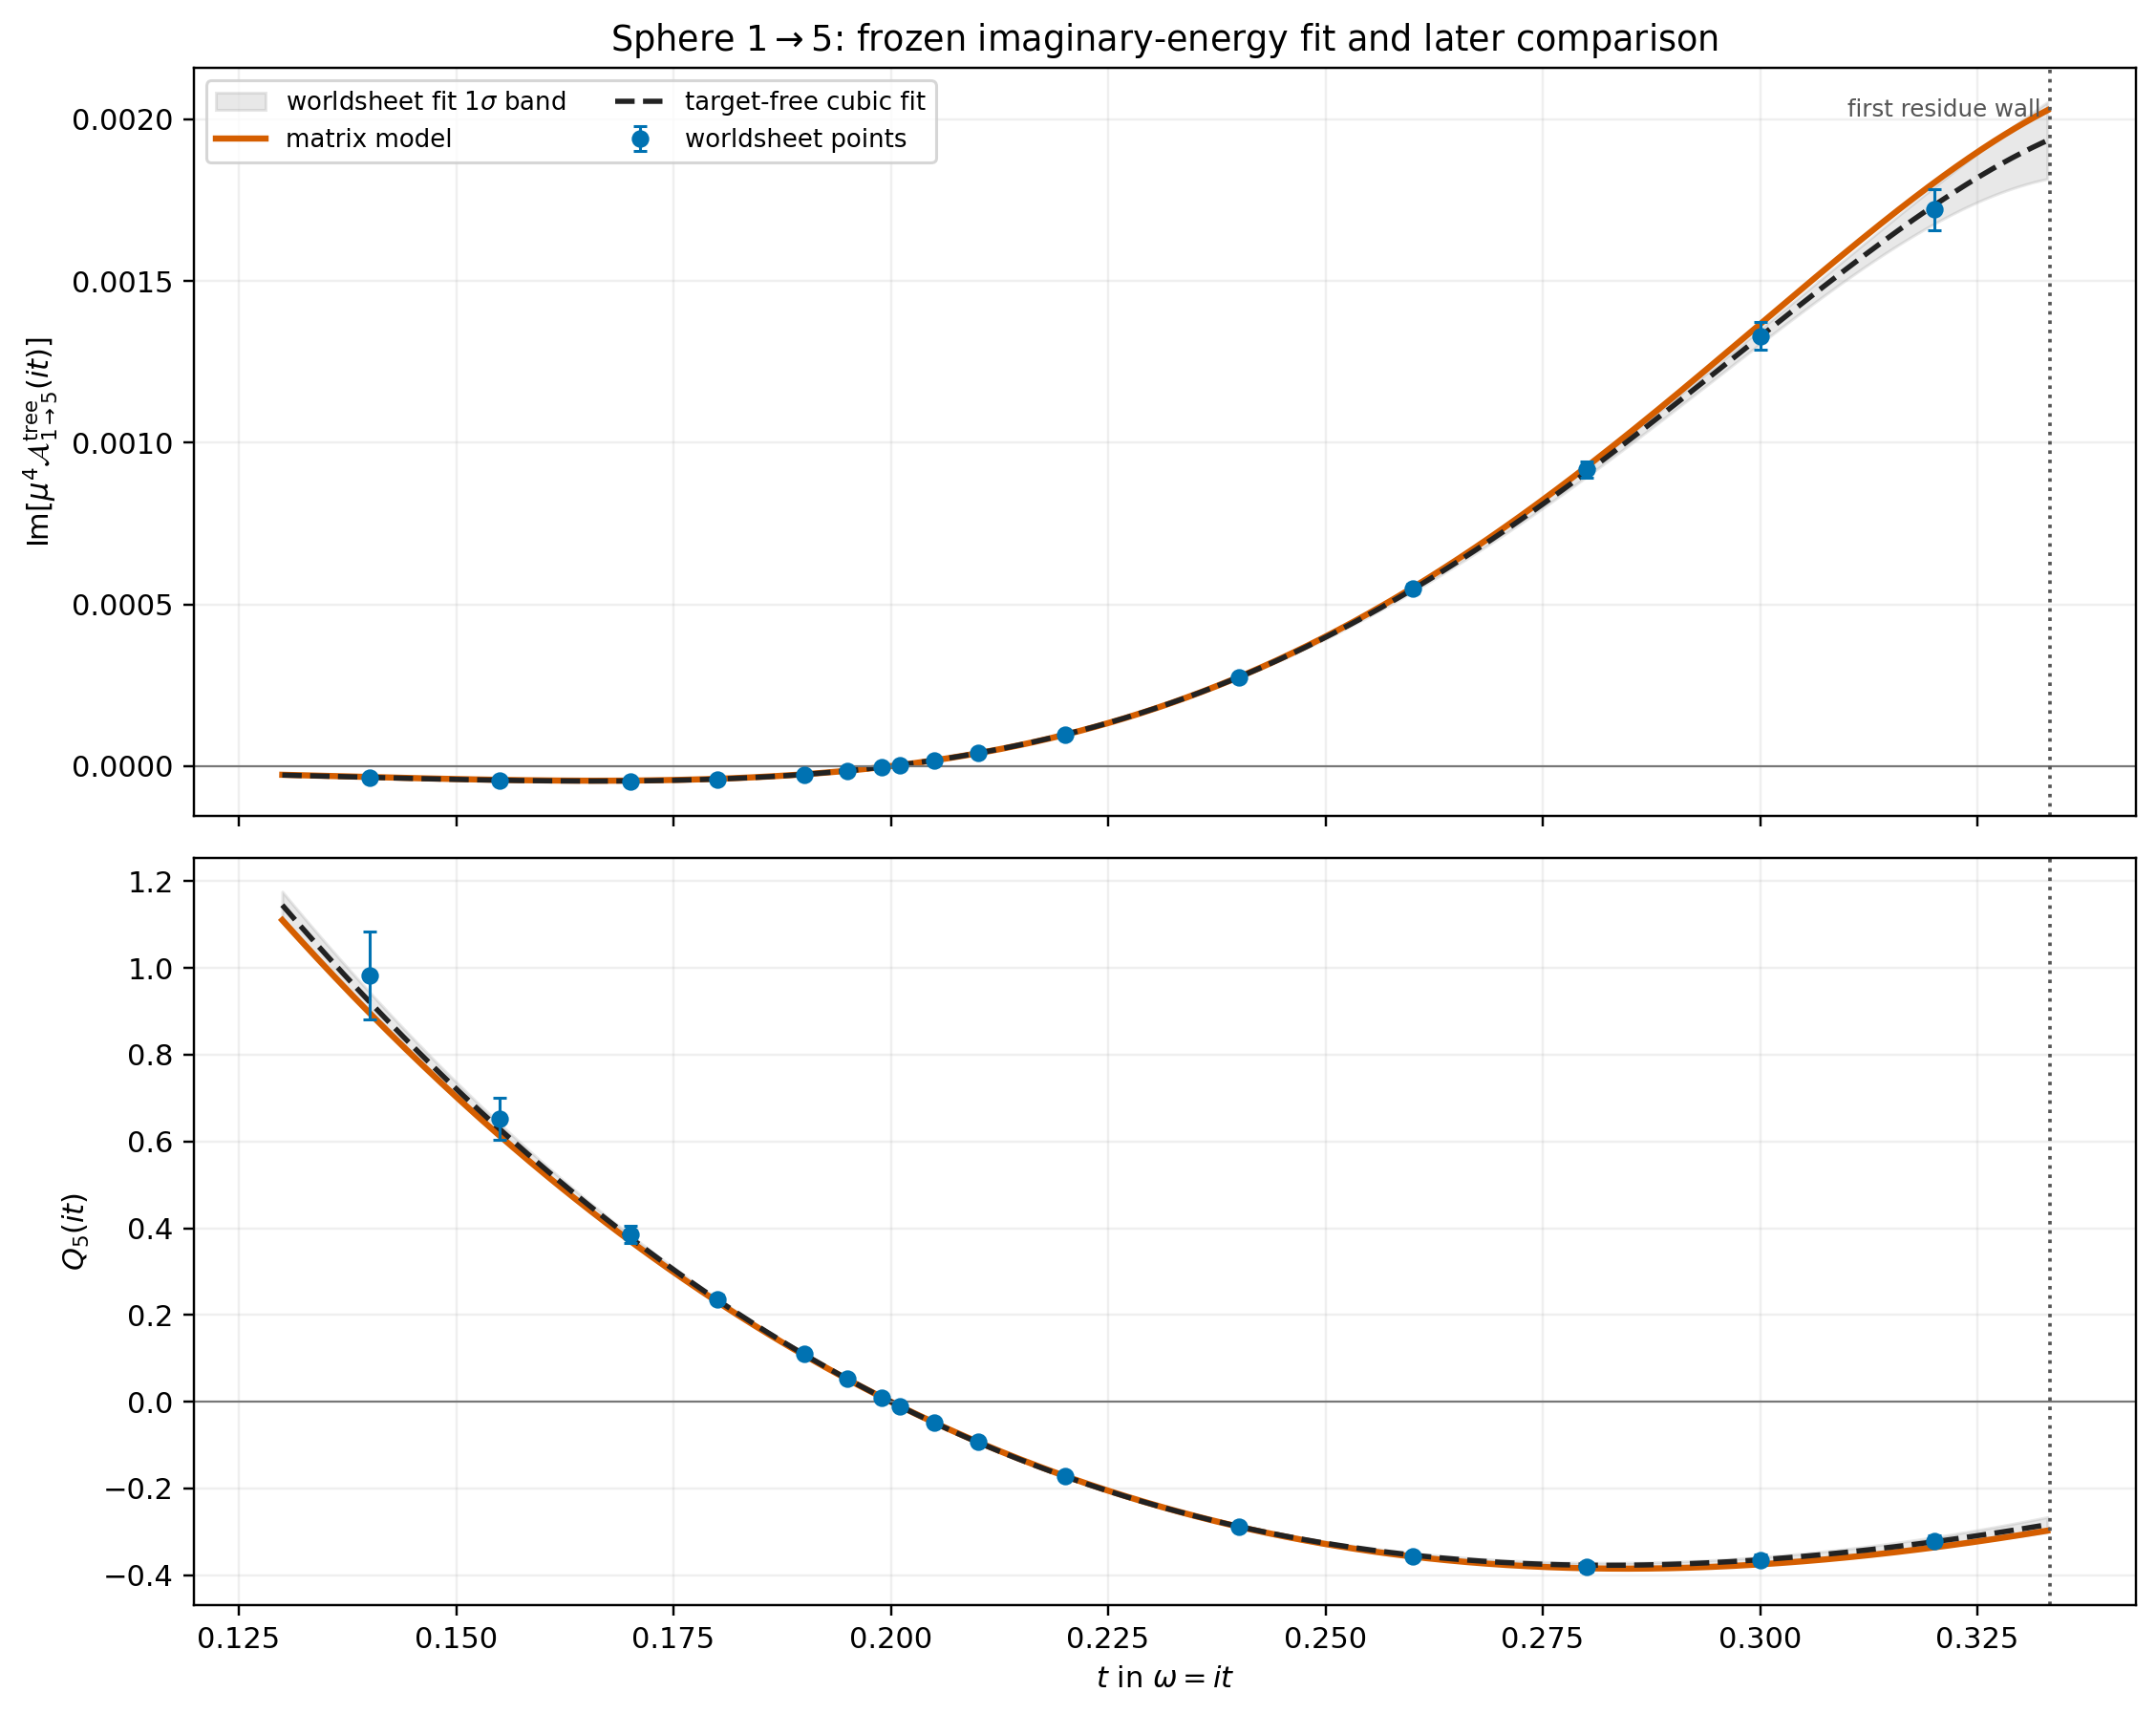
\includegraphics[width=0.94\textwidth]{results/sphere_six_point_1to5/sphere_one_to_five_amplitude_16point_fit.png}
  \caption{Sphere $1\to5$ amplitude at all sixteen local points in the
  residue-free chamber.  Blue circles are the frozen worldsheet values, the
  black dashed curve and grey band are the target-free cubic fit and its
  one-standard-error band, and the orange curve is the matrix-model
  prediction loaded only afterward.  The upper panel shows the imaginary
  part of the normalized amplitude; the lower panel shows $Q_5$.  Displayed
  point errors combine independent scrambled-Sobol QMC errors with
  \eqref{eq:Q5-discretization} in quadrature.  The dotted line marks the first
  Liouville residue wall at $t=1/3$; no data are plotted beyond it.}
  \label{fig:one-to-five-comparison}
\end{figure}

Figure~\ref{fig:one-to-five-comparison} shows separately the result inferred
from imaginary-energy worldsheet data and the later comparison curve.  Their
agreement throughout the chamber, including the independently resolved zero
crossing near $t=0.2$ and the non-monotonic shape of $Q_5$, tests more than an
overall normalization.
\FloatBarrier

\subsubsection{Current thirty-point order-eight comparison}

For the current result, the comparison program first verifies the status and
hash of the target-free order-eight fit and only then loads the matrix-model
coefficient vector $(6,-55,150,-125)$.  The comparison output has SHA-256
hash
\begin{center}
\small\ttfamily
43f8ea67c28cb79fe37ac7c6766b51dc4dcc7c25f9d1c52c1610f6f461f1d86e.
\end{center}

\paragraph{Coefficient-by-coefficient comparison.}
Table~\ref{tab:Q5-order8-coefficients} compares the primary target-free fit
in \eqref{eq:Q5-order8-cubic-fit} with the analytic coefficient vector.  Its
quoted errors are the marginal errors from the propagated-QMC covariance;
they do not contain a block-order-eight-to-higher truncation estimate.

\begin{table}[H]
\centering
\small
\caption{Detailed coefficient comparison for
$Q_5(\ii t)=a+bt+ct^2+dt^3$.  Here
$\Delta=c_{\mathrm{WS}}-c_{\mathrm{MM}}$; the relative difference is signed.}
\label{tab:Q5-order8-coefficients}
\begin{tabular}{@{}c r r r r r@{}}
\toprule
Coefficient & Order-eight worldsheet fit & Matrix model & $\Delta$
& $100\Delta/c_{\mathrm{MM}}$ & $\Delta/\sigma_{\mathrm{stat}}$ \\
\midrule
$a$ & $  6.21496\pm0.10398$ & $   6$ & $ 0.21496$ & $3.583\%$ & $ 2.07$ \\
$b$ & $-56.88322\pm1.30064$ & $ -55$ & $-1.88322$ & $3.424\%$ & $-1.45$ \\
$c$ & $154.63270\pm5.35582$ & $ 150$ & $ 4.63270$ & $3.088\%$ & $ 0.86$ \\
$d$ & $-127.95294\pm7.24154$ & $-125$ & $-2.95294$ & $2.362\%$ & $-0.41$ \\
\bottomrule
\end{tabular}
\end{table}

Thus all four coefficients have the predicted sign, and all four fitted
magnitudes are larger than the analytic magnitudes by between $2.36\%$ and
$3.58\%$.  The differences are therefore close to a coherent overall
normalization shift, rather than four unrelated coefficient distortions.
The largest marginal displacement is the constant term at $2.07$ of its
statistical standard errors.

The four coefficients are nevertheless very strongly correlated.  In the
order $(a,b,c,d)$, the propagated-statistical correlation matrix is
\begin{equation}
 \operatorname{Corr}_{\mathrm{stat}}=
 \begin{pmatrix}
  1       &-0.99849& 0.99382&-0.98644\\
 -0.99849& 1       &-0.99842& 0.99393\\
  0.99382&-0.99842& 1       &-0.99853\\
 -0.98644& 0.99393&-0.99853& 1
 \end{pmatrix}.
 \label{eq:Q5-order8-coefficient-correlation}
\end{equation}
Consequently, the four marginal pulls in
Table~\ref{tab:Q5-order8-coefficients} must not be combined as independent
numbers.  With the full statistical covariance,
\begin{equation}
 \Delta\boldsymbol c^{\mathsf T}C_{\mathrm{stat}}^{-1}
 \Delta\boldsymbol c
 =308.85
 =310.97-2.12.
 \label{eq:Q5-order8-coefficient-joint-stat}
\end{equation}
The last equality is the weighted-least-squares identity: $310.97$ is the
statistical-only pointwise $\chi^2$ of the fixed matrix polynomial and
$2.12$ is that of the fitted cubic.  This large joint statistic is not a
failure of the visual comparison; it says that the QMC error alone is much
smaller than the coherent residual numerical truncation.

Repeating the coefficient extraction with the available numerical-envelope
proxy gives
\begin{align}
 \boldsymbol c_{\mathrm{env}}
   &=(6.19841,-56.67403,153.76488,-126.77468),\\
 \boldsymbol\sigma_{\mathrm{env}}
   &=(0.34893,4.33613,17.73412,23.81823),\\
 \frac{\boldsymbol c_{\mathrm{env}}-\boldsymbol c_{\mathrm{MM}}}
        {\boldsymbol\sigma_{\mathrm{env}}}
   &=(0.57,-0.39,0.21,-0.07).
 \label{eq:Q5-order8-coefficient-envelope}
\end{align}
The corresponding relative differences are
$(3.31\%,3.04\%,2.51\%,1.42\%)$, and the full envelope-weighted coefficient
quadratic form is $28.34=28.55-0.21$.  Because the envelope is a conservative
pointwise numerical proxy and does not model cross-$t$ correlations, neither
this number nor \eqref{eq:Q5-order8-coefficient-joint-stat} is assigned a
formal probability.

\paragraph{Root comparison.}
The factorized matrix polynomial has roots $(0.2,0.4,0.6)$.  The roots of the
target-free order-eight cubic provide a better-conditioned shape diagnostic:
\begin{table}[H]
\centering
\small
\caption{Roots inferred from the target-free order-eight cubic.  Formal
errors use linear propagation of the statistical coefficient covariance.
Only the first root lies inside the sampled interval.}
\label{tab:Q5-order8-roots}
\begin{tabular}{@{}c r r r r l@{}}
\toprule
Root & Worldsheet fit & Matrix model & Difference & Formal pull & Support \\
\midrule
$t_1$ & $0.20000011\pm0.00000562$ & $0.200000$ & $ 1.09\times10^{-7}$ & $ 0.02$ & sampled \\
$t_2$ & $0.397424\pm0.004081$      & $0.400000$ & $-2.58\times10^{-3}$ & $-0.63$ & extrapolated \\
$t_3$ & $0.61109\pm0.03070$        & $0.600000$ & $ 1.11\times10^{-2}$ & $ 0.36$ & extrapolated \\
\bottomrule
\end{tabular}
\end{table}
The first zero is directly resolved in the data and agrees with $t=0.2$ at
the displayed precision.  The other two agree within their formal fit errors
but lie outside both the sampled range and, for $t_2,t_3$, the residue-free
chamber; they are reported only as cubic-extrapolation diagnostics.  The
envelope-weighted roots, $(0.19999999,0.396788,0.616111)$, lead to the same
conclusion.

\paragraph{Pointwise curve comparison.}
On the thirty individual points, using the available order-six numerical
envelope as the conservative uncertainty proxy gives
\begin{equation}
  \chi^2_{\mathrm{env}}=28.55/30,
  \qquad
  \max_k\left|\frac{Q_{5,k}^{(8)}-Q_{5,k}^{\mathrm{expected}}}
                         {\delta Q_{5,k}^{\mathrm{env}}}\right|=1.15,
  \label{eq:Q5-order8-matrix-comparison}
\end{equation}
with RMS pointwise difference $1.06\times10^{-2}$ in $Q_5$.  If only the
propagated QMC errors in \eqref{eq:Q5-paired-order8-error} are retained, the
same comparison gives $\chi^2=310.97/30$ and maximum pull $3.87$.  This
statistical-only diagnostic makes clear that the residual numerical
truncation, not the sampling error, controls the present accuracy.  Thus
\eqref{eq:Q5-order8-matrix-comparison} is a useful conservative comparison,
but not a replacement for the explicitly postponed order-eight-to-higher
certificate.

\begin{figure}[H]
  \centering
  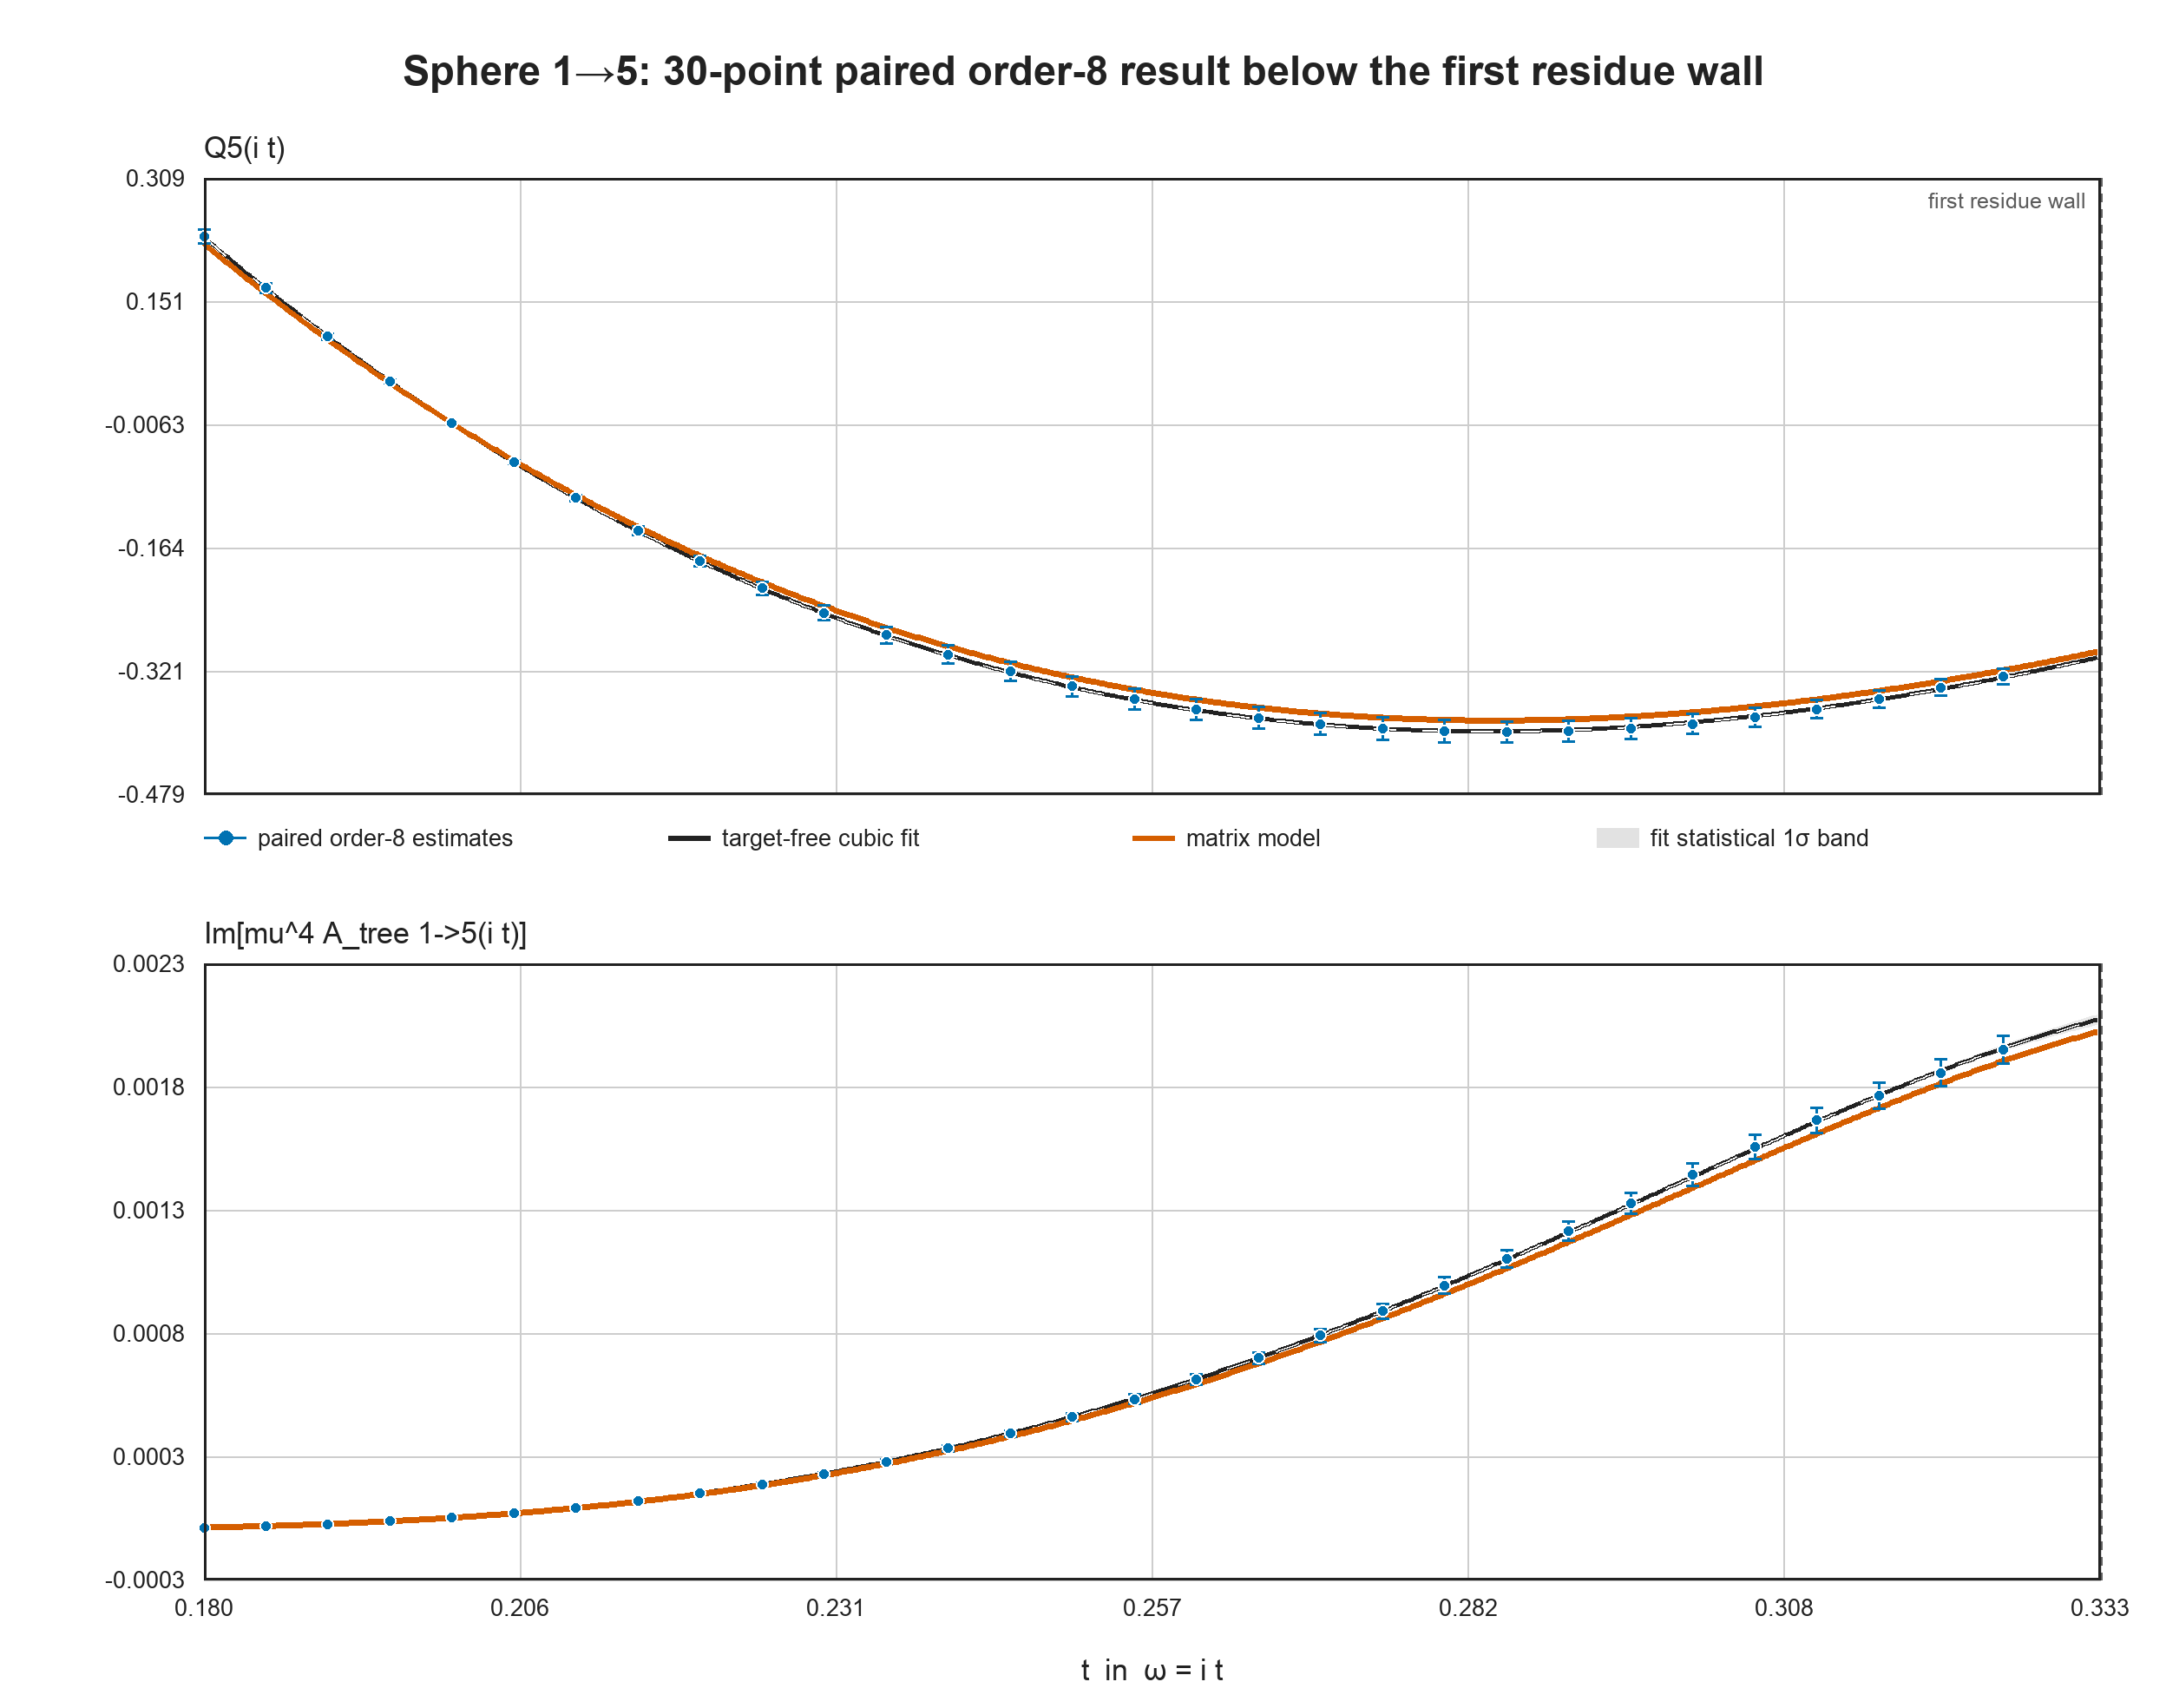
\includegraphics[width=0.96\textwidth]{results/sphere_six_point_1to5/order8_30point_current/sphere_one_to_five_order8_30point_comparison.png}
  \caption{Current sphere $1\to5$ result at thirty points below the first
  residue wall.  Blue points are the paired order-eight estimators in
  \eqref{eq:Q5-paired-order8-estimator}, with error bars equal to the
  available order-six numerical-envelope proxy.  The black dashed curve and
  grey band are the target-free cubic fit and its propagated statistical
  one-standard-error band.  The orange matrix-model curve is evaluated only
  by the separate post-fit comparison.  The panels display $Q_5(\ii t)$ and
  $\operatorname{Im}[\mu^4\A^{\mathrm{tree}}_{1\to5}(\ii t)]$; the dotted
  line marks $t=1/3$.}
  \label{fig:one-to-five-order8-30point}
\end{figure}

The order-eight result in Figure~\ref{fig:one-to-five-order8-30point} is the
current numerical conclusion adopted in this note.  An order-ten upgrade is
not required for the present comparison and has been postponed; Cannon is
reserved for later computations where cluster-scale resources are essential.
\FloatBarrier

\section{Matrix-model pattern after the three comparisons}

After the three process-specific worldsheet calculations and audits have been
fixed, their matrix-model comparison functions can be written in the common
form
\begin{equation}
  \boxed{
  Q_n^{\mathrm{expected}}
  (\omega_{\mathrm{in}};\omega_1,\ldots,\omega_n)
  =\prod_{m=1}^{n-2}(\ii\omega_{\mathrm{in}}+m).}
  \label{eq:expected-Qn}
\end{equation}
For equal outgoing energies, $\omega_{\mathrm{in}}=n\omega$, this gives
\begin{equation}
  \boxed{
  \mu^{n-1}\A^{\mathrm{tree}}_{1\to n}(\omega)
  =\ii n\omega^{n+1}
   \prod_{m=1}^{n-2}(m+\ii n\omega).}
  \label{eq:expected-equal-energy}
\end{equation}
Equations~\eqref{eq:expected-Qn} and
\eqref{eq:expected-equal-energy} summarize the comparison target supported by
the $1\to3$, $1\to4$, and $1\to5$ data.  They are not inputs to any of the
worldsheet integrations and do not constitute a worldsheet proof at arbitrary
multiplicity.

\section{A scalable route to general \texorpdfstring{$1\to n$}{1 to n}}

A sphere $1\to n$ amplitude is an $(n+1)$-point correlator.  A trivalent
channel contains
\begin{equation}
  (n+1)-3=n-2
\end{equation}
internal Liouville momenta.  A scalable computation should separate the
discrete contour bookkeeping from the numerical contraction of the
continuous integrals.

\subsection{Momentum-contour forest}

For every trivalent vertex:
\begin{enumerate}
  \item construct the affine DOZZ pole hyperplanes in the adjacent internal
  momenta and external energies;
  \item determine which hyperplanes cross the declared contours as the
  external energies move;
  \item add the residues with their oriented signs;
  \item inspect each residue integrand recursively for further crossings;
  \item organize simultaneous crossings as lower-dimensional residue
  strata.
\end{enumerate}
Within a fixed kinematic chamber, the answer becomes a sum of integrals of
dimensions
\begin{equation}
  n-2,\ n-3,\ \ldots,\ 0.
\end{equation}
This ``contour forest'' is the higher-point version of the single residue in
\eqref{eq:residue-prescription}.

\subsection{Quadrature and tensor contraction}

Each continuous or residue stratum should use:
\begin{itemize}
  \item a Gauss--Jacobi threshold panel after the exact small-$P$ power has
  been factored out;
  \item ordinary bulk panels divided at nearby pole projections and pole
  widths;
  \item a separate Gaussian-tail or rationally mapped tail panel;
  \item a threshold block evaluator that avoids nearly degenerate
  fixed-weight $c$-recursion nodes.
\end{itemize}

At fixed plumbing coordinates, the trivalent tree is naturally a tensor
network.  Momentum nodes are edge indices, DOZZ and descendant couplings are
vertex tensors, and plumbing powers are diagonal edge tensors.  Contracting
the tree locally avoids an explicit $M^{n-2}$ tensor grid.  Without further
compression, the generic cost is of order
\begin{equation}
  O(nM^3).
\end{equation}

\section{Error budget and limitations}

For every future $1\to n$ production point, the following uncertainties
should be retained separately:
\begin{enumerate}
  \item adjacent momentum rules and threshold refinements;
  \item adjacent Virasoro-block orders;
  \item moduli QMC depth and independent scrambles;
  \item agreement between overlapping OPE channels;
  \item distance to the next momentum-contour wall;
  \item residue-stratum quadrature;
  \item any rational-reconstruction or degree assumption.
\end{enumerate}

The present $1\to3$, $1\to4$, and $1\to5$ evidence identifies the corresponding
analytic answers very strongly in controlled imaginary-energy chambers.  It
is not, by itself, a theorem that $Q_4$ has degree two or that $Q_5$ has
degree three.  Nor does it yet constitute a worldsheet derivation of
\eqref{eq:expected-Qn} for arbitrary $n$.

\appendix
\section{Machine-readable provenance and implementation map}
\label{sec:code-map}

This appendix is a reviewer-oriented map of the code that directly supports
the sphere $1\to n$ claims.  File names are relative to the \path{plumbing/}
directory.  The self-contained review snapshot is generated by
\path{build_sphere_one_to_n_review_bundle.py}; its manifest follows all local
Python imports and therefore includes shared transitive dependencies not
listed individually below.

\subsection{Trust boundary used in every blind calculation}

The production flow is deliberately split into files with different
authority:
\begin{enumerate}
  \item a worldsheet kernel evaluates Liouville structure constants,
  timelike factors, conformal blocks, and moduli weights;
  \item a worldsheet scan produces raw integrals and stripped amplitudes but
  contains no target polynomial;
  \item an audit varies numerical settings and is also target-blind;
  \item the worldsheet JSON is hashed and frozen;
  \item only a separate comparison file imports or evaluates the
  matrix-model function, after verifying the frozen hashes.
\end{enumerate}
This boundary is enforced explicitly for all three cases.  In the current
$1\to4$ path, the twelve-point extension is produced without a target
polynomial, the merger verifies the historical points and extension hashes,
and the target-free fitter freezes the thirty-point table and
twenty-nine-point primary fit.  Only then does the downstream comparison
verify those hashes and evaluate the matrix coefficients.  The earlier
eighteen-point fit is retained only as input-lineage provenance and is not a
competing result in this note.
The $1\to5$ path applies the same separation both to its earlier sixteen
residue-free points and to the current thirty-point paired order-eight
estimator.  The completed Cannon source declares that no target formula was
available; the order-eight fit program contains no comparison coefficient;
and the separate comparison accepts only the resulting target-free status.

\subsection{Shared normalization, Liouville input, and blocks}

\begin{description}[style=nextline,leftmargin=2.8cm]
  \item[Normalization]
  \path{audit_genus0_one_to_two_amplitude.py} derives the sphere normalization
  from the three-point anchor; \path{audit_genus0_one_to_two_amplitude_checks.py}
  is its regression gate.  \path{audit_c1_sphere_topology_normalization.py}
  and its check file provide an independent topology-normalization ledger.

  \item[Liouville data]
  \path{liouville_torus.py} implements $\Upsilon_1$, the logarithmic
  delta-normalized DOZZ/Yin structure constant, and shared special-function
  conventions.  \path{liouville_torus_checks.py} tests reflection,
  shift, and normalization identities.  No matrix-model information enters
  this layer.

  \item[Virasoro blocks]
  \path{ccy_sphere_four_point.py}, \path{ccy_sphere_five_point.py},
  \path{ccy_sphere_six_point.py}, and
  \path{ccy_sphere_six_point_star.py} implement the four-, five-, and
  six-point CCY recursions in the channel coordinates used by the moduli
  atlases.  Each has a corresponding \path{*_checks.py} file.  The checks
  compare low levels with direct descendant sums, verify elliptic-nome
  re-expansion, exchange symmetries, and comb--star factorization limits.
\end{description}

\subsection{Sphere \texorpdfstring{$1\to3$}{1 to 3} code path}

\begin{description}[style=nextline,leftmargin=3.8cm]
  \item[Convergent kernel]
  \path{sphere_four_point_imaginary_energy.py} fixes $\omega=\ii t$,
  constructs the one-momentum Liouville kernel, and implements the exact
  three-chart proposal \eqref{eq:Q3-three-chart-proposal}.

  \item[Blind production]
  \path{sphere_four_point_worldsheet_scan.py}\par
  evaluates both the original
  sixteen-point table and the fourteen-point interlaced extension, records
  all replicate estimates and settings, and writes their frozen hashes.

  \item[Blind merge and fit]
  \path{merge_sphere_four_point_worldsheet_scans.py} verifies the original
  and extension hashes, common numerical design, disjoint seed streams, and
  interlaced kinematics before freezing the thirty-point table.
  \path{sphere_four_point_imaginary_ray_fit.py} then freezes the primary,
  cohort, and deep-audit-replacement affine fits without importing a target
  coefficient.

  \item[Blind convergence]
  \path{sphere_four_point_worldsheet_audit.py} verifies the production hash
  before varying block order, momentum order, cutoff, and RQMC depth.  It
  produced a four-point audit and a separate deep audit at $t=0.32$.

  \item[Later comparison]
  \path{sphere_four_point_30point_matrix_comparison.py}\par
  contains the new
  thirty-point $Q_3^{\mathrm{expected}}$ comparison.  It refuses mismatched
  scan or fit hashes and produces the cohort diagnostics and
  \path{amplitude_comparison_30point.png}.\par
  The earlier \path{sphere_four_point_matrix_comparison.py}\par
  remains the frozen
  sixteen-point comparison record.

  \item[Physical control branch]
  \path{sphere_four_point_physical.py} and
  \path{sphere_four_point_subtraction.py} implement the independent physical
  $i\epsilon$ BRY finite part.  Their check files verify collar independence,
  local projector cancellation, energy conservation, and the published
  four-point benchmark.  This branch shares block and DOZZ primitives but is
  not used to generate the imaginary-ray production table.
\end{description}

The inherited audit artifacts are
\path{results/sphere_four_point_1to3/worldsheet_audit.json} and
\path{results/sphere_four_point_1to3/worldsheet_audit_t032.json}.  The new
thirty-point artifacts reside in
\begin{center}
\small\path{results/sphere_four_point_1to3/blind30_20260824/}
\end{center}
Its principal files are
\begin{itemize}
  \item \path{worldsheet_extension_14point.json};
  \item \path{worldsheet_scan_30point.json};
  \item \path{worldsheet_affine_fit_30point_frozen.json};
  \item \path{matrix_comparison_30point.json}.
\end{itemize}

\subsection{Sphere \texorpdfstring{$1\to4$}{1 to 4} code path}

\begin{description}[style=nextline,leftmargin=3.8cm]
  \item[Geometry and Liouville]
  \path{sphere_five_point_liouville.py} constructs labelled five-point
  channels, their Jacobians, and Liouville factors;
  \path{sphere_five_point_liouville_checks.py} tests channel overlap and
  covariance.

  \item[Main kernel and atlas]
  \path{sphere_five_point_equal_energy.py} precomputes the double-momentum
  kernel, evaluates the 120 oriented plumbing charts, implements the exact
  atlas-mixture density, and contains both the subtraction-free and physical
  forest estimators.

  \item[Contour continuation]
  \path{sphere_five_point_extended_scan.py} evaluates the imaginary ray with
  the continued real contour and the $-2\ii$ crossed-pole residue above
  $t=2/5$.  \path{sphere_five_point_continuation_checks.py} tests the residue
  and its chamber of validity.

  \item[Physical finite part]
  \path{sphere_five_point_subtraction.py},
  \path{sphere_five_point_physical_scan.py}, and their check files implement
  and test the physical BRY forest independently of the convergent-ray scan.
  This branch remains a smoke test and supplies no curve used in this note.

  \item[Thirty-point production and fit]
  \path{sphere_five_point_30point_worldsheet_extension.py}\par
  computes and freezes the twelve new points with disjoint Sobol seed blocks.
  \path{sphere_five_point_30point_worldsheet_fit.py}\par
  verifies the historical table and extension hashes, merges all thirty
  points, and performs the target-free quadratic fits.  Neither file contains
  a matrix-model coefficient.

  \item[Worldsheet audit]
  \path{sphere_five_point_30point_audit_summary.py} freezes the independent
  block-order checks at $t=0.31,0.35,0.44$ and constructs the conservative
  local uncertainties.  The full regression and lineage gate is
  \path{sphere_five_point_30point_checks.py}.

  \item[Later comparison]
  \path{sphere_five_point_30point_matrix_comparison.py}\par
  accepts only the frozen thirty-point scan, fit, and audit, verifies their
  hashes, and then evaluates the matrix-model coefficients and produces
  Figure~\ref{fig:amplitude-comparison}.
  \path{sphere_five_point_numerical_recipe.md}\par
  records the two distinct imaginary-ray and direct-physical prescriptions.
  \path{sphere_n_point_momentum_integration.md}\par
  records the general momentum strategy.
\end{description}

The only current $1\to4$ result artifacts used in this note reside in
\begin{center}
\small\path{results/sphere_five_point_1to4/blind30_20260824/}
\end{center}
Their principal files are
\begin{itemize}
  \item \path{worldsheet_extension_12point.json};
  \item \path{worldsheet_scan_30point.json};
  \item \path{worldsheet_points_30point_frozen.json};
  \item \path{worldsheet_quadratic_fit_30point_frozen.json};
  \item \path{worldsheet_newpoint_block_audit_frozen.json};
  \item \path{matrix_comparison_30point.json};
  \item \path{amplitude_comparison_30point.png}.
\end{itemize}

\subsection{Sphere \texorpdfstring{$1\to5$}{1 to 5} code path}

\begin{description}[style=nextline,leftmargin=3.8cm]
  \item[Six-point atlases]
  \path{sphere_six_point_atlas.py} enumerates 720 labelled comb and 720
  labelled star charts, maps their plumbing variables to puncture positions,
  computes Jacobians, and evaluates the full mixture density.
  \path{sphere_six_point_atlas_checks.py} verifies coverage, label counting,
  Jacobians, and overlap transformations.

  \item[Worldsheet kernel]
  \path{sphere_six_point_equal_energy.py} constructs the cached
  three-momentum DOZZ tensor, selects the appropriate comb or star block,
  evaluates the timelike factor, and contracts the block at every moduli
  point.  \path{sphere_six_point_equal_energy_pilot.py} fixes the first wall
  and benchmarks block cost; it is not a production substitute.

  \item[Production/audit]
  \path{sphere_six_point_worldsheet_scan.py} is the target-blind production
  driver.  \path{sphere_six_point_worldsheet_audit.py} performs momentum,
  block, cutoff, radial-sampler, and channel diagnostics without importing
  the prediction.

  \item[Extension/merge]
  The same scan driver produced the later eight local points.
  \path{merge_sphere_six_point_worldsheet_scans.py} verifies distinct points,
  chamber membership, zero fallback counts, and settings compatibility before
  writing and freezing the sixteen-point merged table.

  \item[Imaginary-ray fit]
  \path{sphere_six_point_imaginary_ray_fit.py} verifies the merged scan and
  its original freeze, writes a target-free points-only table, and performs
  the cubic GLS fit in \eqref{eq:Q5-worldsheet-fit-ansatz}.  Its regression and
  trust-boundary gate is
  \path{sphere_six_point_imaginary_ray_fit_checks.py}.

  \item[Current order-eight fit]
  \path{sphere_six_point_order8_current_fit.py} verifies the exact completed
  thirty-point source hash, checks that the source contains no target, forms
  the paired estimator \eqref{eq:Q5-paired-order8-estimator}, and performs the
  cubic fit without a matrix-model coefficient.  Its source is
  \path{results/sphere_six_point_1to5/cannon_blind30_3h_v2/assembled/}
  \path{worldsheet_scan_unfrozen.json}.  The ``unfrozen'' file name records
  failure of the original strict order-six accuracy gate; it does not mean
  that the source values are mutable or that target information is present.

  \item[Later comparison]
  \path{sphere_six_point_imaginary_ray_fit_comparison.py} verifies the frozen
  fit and its source-point hash before evaluating the expected $Q_5$
  polynomial and producing Figure~\ref{fig:one-to-five-comparison}.
  \path{sphere_six_point_matrix_comparison.py} retains the earlier direct
  pointwise comparison as an independent consistency artifact.
  \path{sphere_six_point_order8_current_comparison.py} is the separate
  current comparison; it accepts only the target-free order-eight status and
  produces Figure~\ref{fig:one-to-five-order8-30point}.

  \item[Cannon campaign]
  \path{sphere_six_point_cannon_blind.py},
  \path{sphere_six_point_cannon_compare_after_freeze.py}, their checks, the
  \path{config/sphere_six_point_1to5_cannon_blind50_v1.json} configuration,
  and the \path{cluster/sphere_six_point_1to5_blind_*.slurm} scripts are
  infrastructure for the requested 50-point high-accuracy campaign.  That
  campaign was cancelled.  The corrected replacement campaign under
  \path{results/sphere_six_point_1to5/cannon_blind30_3h_v2/} completed all
  450 target-blind production and paired-systematics shards after exact
  recovery of rare source-chart $q=0$ roundoff cases.  Its strict
  $5\times10^{-4}$ order-six gate did not pass because the paired block
  correction was resolved; the present analysis incorporates that correction
  as the order-eight estimator instead of discarding it.

  A first block-order-ten trial was submitted as jobs 41589119, 41589131,
  41589136, and 41589138.  Its production validation task completed, its
  high-order systematics validation task exhausted memory, and every
  dependent job was cancelled.  No order-ten number from that attempt is
  used here.  The files
  \path{sphere_six_point_cannon_block10_upgrade.py} and
  \path{config/sphere_six_point_1to5_cannon_block10_upgrade_v2.json} preserve
  a possible lower-memory redesign, but it was not submitted.  The
  order-ten upgrade is now postponed and there is no active Cannon job for
  this project.
\end{description}

The principal $1\to5$ artifacts are
\begin{itemize}
  \item \path{results/sphere_six_point_1to5/worldsheet_convergent_scan.json};
  \item \path{results/sphere_six_point_1to5/worldsheet_convergent_scan_extension8_local.json};
  \item \path{results/sphere_six_point_1to5/worldsheet_convergent_scan_16point_local.json};
  \item \path{results/sphere_six_point_1to5/worldsheet_freeze_manifest_16point_local.json};
  \item \path{results/sphere_six_point_1to5/worldsheet_numerical_audit.json};
  \item \path{results/sphere_six_point_1to5/worldsheet_imaginary_ray_points_frozen.json};
  \item \path{results/sphere_six_point_1to5/worldsheet_imaginary_ray_cubic_fit_frozen.json};
  \item \path{results/sphere_six_point_1to5/matrix_model_fit_comparison_16point_local.json}.
  \item \path{results/sphere_six_point_1to5/cannon_blind30_3h_v2/assembled/}
        \path{worldsheet_scan_unfrozen.json};
  \item \path{results/sphere_six_point_1to5/order8_30point_current/}
        \path{order8_target_free_fit.json};
  \item \path{results/sphere_six_point_1to5/order8_30point_current/}
        \path{order8_matrix_comparison.json};
  \item \path{results/sphere_six_point_1to5/order8_30point_current/}
        \path{sphere_one_to_five_order8_30point_comparison.png}.
\end{itemize}

\subsection{Recommended faithfulness-review order}

The shortest review path that still checks every conceptual boundary is:
\begin{enumerate}
  \item verify the labelled normalization with
  \path{audit_genus0_one_to_two_amplitude.py};
  \item inspect \path{liouville_torus.py} and its special-function checks;
  \item run the four-, five-, and six-point CCY block checks;
  \item inspect the exact proposal-mixture densities in the $1\to3$ kernel,
  five-point equal-energy kernel, and six-point atlas;
  \item trace one integrand from external energies through DOZZ tensors,
  block evaluation, timelike factor, Jacobian, and proposal weight;
  \item verify the frozen JSON hashes independently;
  \item confirm by source inspection that worldsheet scan and audit files do
  not import comparison modules or contain target polynomials;
  \item only then run the process-specific matrix-comparison files, including
  the separate current order-eight $1\to5$ comparison.
\end{enumerate}

\end{document}
